\documentclass[preprintnumbers,prd,superscriptaddress,preprint]{revtex4-1}

\usepackage{CJK}
\usepackage{amsmath}
\usepackage{subfigure}
\usepackage{enumerate}
\usepackage{amssymb}
\usepackage{amsfonts}
\usepackage{mathrsfs}
\usepackage{latexsym}
\usepackage{bm}
\usepackage{amscd}
\usepackage{physics} 
\usepackage{graphicx}
\usepackage{epsfig}
\usepackage{hhline,multirow}
\usepackage{dcolumn}
\usepackage{url}
\usepackage[colorlinks=true,linkcolor=blue,citecolor=blue,urlcolor=blue]{hyperref}
\usepackage{color}
\usepackage{soul}
\usepackage{xcolor}
\usepackage{indentfirst}
\usepackage{subfigure}
\usepackage{psfrag}
\usepackage{slashed}
\usepackage{float}
\usepackage{setspace}
\usepackage{empheq}
\usepackage{mathtools}
\usepackage{cancel}
\allowdisplaybreaks[2]

\begin{document}
	\title{unpolarize GPD draft}
	
	\author{Zhengyang Gao}
	\affiliation{Institute of High Energy Physics, Chinese Academy of Sciences,
		Beijing 100049, China}
	\affiliation{\mbox{College of Physics Sciences, University of Chinese Academy of Sciences, Beijing 100049, China}}
	\author{Fangcheng He}% \thanks{fangcheng.he@stonybrook.edu}
	\affiliation{Department of Physics and Astronomy, Stony Brook University, Stony Brook, New York 11790, USA}
	\author{Chueng-Ryong~Ji}
	\affiliation{{Department of Physics, North Carolina State University,
			Raleigh, North Carolina 27695, USA}}
	\author{W. Melnitchouk}
	\affiliation{Jefferson Lab, Newport News, Virginia 23606, USA}
	\author{Y.~Salamu}
	\affiliation{{School of Physics and Electrical Engineering, Kashi University, Kashi, 844000, Xinjiang, China}}
	\author{P. Wang}
	\affiliation{Institute of High Energy Physics, Chinese Academy of Sciences,
		Beijing 100049, China}
	\affiliation{\mbox{College of Physics Sciences, University of Chinese Academy of Sciences, Beijing 100049, China}}
	
	\begin{abstract}
	\end{abstract}
	
	\date{\today}
	\maketitle
	
	\section{Introduction}
	
	\section{Theoretical framework}
	
	\section{Definition of GPD and splitting function}
	
	The unpolarized GPD in our calculation is defined as
	\begin{multline}
		\frac{1}{2}\int\frac{d\lambda}{2\pi}e^{ixP\lambda n_{-}}<p_{2}|\bar{q}(-\frac{1}{2}\lambda n_{-})\cancel{n}_{-}q(\frac{1}{2}\lambda n_{-})|p>\\
		=\frac{1}{2(Pn_{-})}[H^{q}(x,\xi,t)\bar{u}(p_{2})\cancel{n}_{-}u(p_{1})+E^{q}(x,\xi,t)\bar{u}(p_{2})\frac{i\sigma^{\alpha\beta}\cancel{n}_{-\alpha}q_{\beta}}{2M}u(p_{1})]
	\end{multline}
	
	And we use this definition of splitting function 
	\begin{align}
		\bar{u}(p_{2})\Gamma^{+}u(p_{1}) & =\bar{u}(p_{2})[\gamma^{+}f(y,\xi,t)+\frac{i\sigma^{+\alpha}q_{\alpha}}{2M_{B}}g(y,\xi,t)]u(p_{1})\\
		& =\bar{u}(p_{2})[\gamma^{+}(f(y,\xi,t)+g(y,\xi,t))-\frac{p_{1}^{+}+p_{2}^{+}}{2M_{B}}g(y,\xi,t)]u(p_{1})
	\end{align}
	In second line we use 
	\begin{align}
		\frac{i\sigma^{+\alpha}q_{\alpha}}{2M_{B}}=\gamma^{+}-\frac{p_{1}^{+}+p_{2}^{+}}{2M_{B}}
	\end{align}
	
	In order to get the splitting function $f\ g$ from $\Gamma^{+}$ defined in the equation above, we define these two terms. 
	\begin{align}
		A & =\textrm{Tr}[\Gamma^{+}(\cancel{p_{1}}+M_{B})\gamma^{+}(\cancel{p_{2}}+M_{B})]\\
		& =(f(y,\xi,t)+g(y,\xi,t))*\textrm{Tr}[\gamma^{+}(\cancel{p_{1}}+M_{B})\gamma^{+}(\cancel{p_{2}}+M_{B})]\\
		& -\frac{p_{1}^{+}+p_{2}^{+}}{2M_{B}}g(y,\xi,t)*\textrm{Tr}[(\cancel{p_{1}}+M_{B})\gamma^{+}(\cancel{p_{2}}+M_{B})]\\
		B & =\textrm{Tr}[\Gamma^{+}(p_{1}+M_{B})(\cancel{p_{2}}+M_{B})]\frac{p_{1}^{+}+p_{2}^{+}}{2M_{B}}\\
		& =(f(y,\xi,t)+g(y,\xi,t))*\textrm{Tr}[\gamma^{+}(p_{1}+M_{B})(\cancel{p_{2}}+M_{B})]\frac{p_{1}^{+}+p_{2}^{+}}{2M_{B}}\\
		& -\frac{p_{1}^{+}+p_{2}^{+}}{2M_{B}}g(y,\xi,t)*\textrm{Tr}[\gamma^{+}(p_{1}+M_{B})(\cancel{p_{2}}+M_{B})]\frac{p_{1}^{+}+p_{2}^{+}}{2M_{B}}
	\end{align}
	The $f\ g$ in form of$A\ B$ is 
	\begin{align}
		f= & \frac{4M_{B}^{2}\xi^{2}B-Q^{2}A}{8P^{+2}(4M_{B}^{2}\xi^{2}+(\xi^{2}-1)Q^{2})}\\
		g= & \frac{M_{B}^{2}(1-\xi^{2})B-M_{B}^{2}A}{2P^{+2}(4M_{B}^{2}\xi^{2}+(\xi^{2}-1)Q^{2})}
	\end{align}
	
	\section{nonzero skewness splitting function }
	Based on the nonlocal ChPT, the one loop Feynman diagrams contribute to proton's unpolarized GPD are listed in Fig.~\ref{fig:diagrams} 
	
	\begin{figure}[H]
		\begin{center}
			\includegraphics[scale=1]{feynmanndiagrams.pdf}
			\caption{One-loop diagrams for the proton to pseudoscalar meson (dashed lines) and octet baryon (solid lines) or decuplet baryon (double solid lines) splitting functions. The crossed circles ($\otimes$) represent the interaction with the external vector field from the minimal substitution, and the black square (${\textcolor{black}{\blacksquare}}$) denotes the magnetic interaction with the external vector field. The black dot ($\bullet$) is the addition vertex in Kroll-Ruderman diagram.} 
			\label{fig:diagrams}
		\end{center}
	\end{figure}
	
	\subsection{rainbow diagram with octet intermediate state}
	For these diagrams in Fig.~\ref{fig:rainbowdiagrams} we list their contribution to splitting function below.
	
	\begin{figure}[htbp]
		\begin{center}
			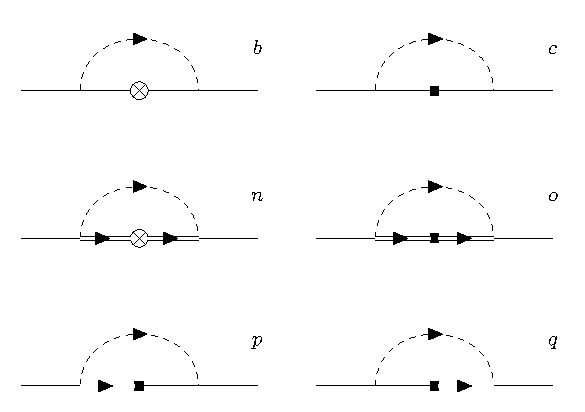
\includegraphics[scale=1]{baryonloop.pdf}
			\caption{Rainbow diagrams where ther external field couples to the baryon loop.} 
			\label{fig:rainbowdiagrams}
		\end{center}
	\end{figure}
	
	\subsubsection{diagram b}
	
	For diagram b in Fig1, the contribution of this diagram is 
	\begin{align}
		\Gamma_{b}^{+}=\frac{C_{B\phi}^{2}}{f^{2}}\int\frac{d^{4}k}{(2\pi)^{4}}\cancel{k}\gamma_{5}\widetilde{F}^{2}(k)\frac{i}{D_{\phi}(k)}\frac{i(\cancel{p_{2}}-\cancel{k}+M_{B})}{D_{B}(p_{2}-k)}\gamma^{+}\frac{i(\cancel{p_{1}}-\cancel{k}+M_{B})}{D_{B}(p_{1}-k)}\cancel{k}\gamma_{5}\delta(y-\frac{k^{+}}{P^{+}})   
	\end{align}
	
	
	where the propagators are defined as 
	\begin{align*}
		D_{\phi}(k) & =k^{2}-m_{\phi}^{2}+i\epsilon\\
		D_{B}(p) & =p^{2}-M_{B}^{2}+i\epsilon
	\end{align*}
	
	the $M_{B}$ and $m_{\phi}$ are the mass of baryon and meson and
	$\widetilde{F}(k)$ is the regulator in ChPT which we chose as 
	\[
	\widetilde{F}(k)=\left(\frac{\Lambda^{2}-m_{\phi}^{2}}{\Lambda^{2}-k^{2}}\right)^{2}
	\]
	
	The splitting function from this diagram contains $\delta$ term 
	\[
	f(y,\xi,t)+f_{\delta}(\xi,t)\delta(y)
	\]
	\[g(y,\xi,t)+g_{\delta}(\xi,t)\delta(y)
	\]
	The first splitting function $f(y,\xi,t)$ and $g(y,\xi,t)$ above are obtained by calculating the integral through residue theory. The $\delta$ term like $f_{\delta}(\xi,t)\delta(y)$ exists because when $k^{+}=0$ the integral over $k^{-}$ gives a divergence which is equal to a $\delta$ function of $k^{+}$.
	
	
	\subsubsection{diagram c }
	
	For diagram c in fig.1, the diagram with magnetic vertex, the amplitude
	is similar to diagram b which is
	\begin{align}
		\Gamma_{c}^{+}=\frac{C_{B\phi}^{2}}{f^{2}}\int\frac{d^{4}k}{(2\pi)^{4}}\cancel{k}\gamma_{5}\widetilde{F}^{2}(k)\frac{i}{D_{\phi}(k)}\frac{i(\cancel{p_{2}}-\cancel{k}+M_{B})}{D_{B}(p_{2}-k)}\frac{i\sigma^{+\nu}q_{\nu}}{2M_{B}}\frac{i(\cancel{p_{1}}-\cancel{k}+M_{B})}{D_{B}(p_{1}-k)}\cancel{k}\gamma_{5}\delta(y-\frac{k^{+}}{P^{+}})
	\end{align}
	
	
	\subsection{rainbow diagram with decuplet intermediate state}
	
	\subsubsection{diagram n}
	
	For diagram n, the rainbow diagram with decuplet intermediate state,
	the contribution of this diagram to splitting function is 
	
	\begin{align*}
		\Gamma_{n}^{+}= & \frac{C_{T\phi}^{2}}{f^{2}}\int\frac{d^{4}k}{(2\pi)^{4}}k_{\lambda}\Theta^{\lambda\sigma}\tilde{F}(k)\frac{i}{D_{\phi}(k)}\frac{i(\cancel{p_{2}}-\cancel{k}+M_{B})}{D_{B}(p_{2}-k)}\\
		& S_{\sigma\alpha}(p'-k)\gamma^{\alpha\beta+}\frac{i(\cancel{p_{1}}-\cancel{k}+M_{B})}{D_{B}(p_{1}-k)}S_{\beta\rho}(p-k)\Theta^{\rho\nu}k_{\nu}\tilde{F}(k)\delta(y-\frac{k^{+}}{P^{+}})
	\end{align*}
	
	
	\subsubsection{diagram o}
	
	For diagram o, which contains the magnetic interaction between photon
	with decuplet baryon, the contribution is 
	
	\begin{align*}
		\Gamma_{o}^{+}= & \frac{C_{T\phi}^{2}}{f^{2}}\int\frac{d^{4}k}{(2\pi)^{4}}k_{\lambda}\Theta^{\lambda\sigma}\tilde{F}(k)\frac{i}{D_{\phi}(k)}\frac{i(\cancel{p_{2}}-\cancel{k}+M_{B})}{D_{B}(p_{2}-k)}S_{\sigma\alpha}(p'-k)\frac{i\sigma^{+\nu}q_{\nu}}{2M_{B}}\frac{i(\cancel{p_{1}}-\cancel{k}+M_{B})}{D_{B}(p_{1}-k)}\\
		& S_{\alpha\rho}(p-k)\Theta^{\rho\nu}k_{\nu}\tilde{F}(k)\delta(y-\frac{k^{+}}{P^{+}})
	\end{align*}
	
	
	\subsection{transition diagram}
	
	The diagram p and q are the transition diagrams with a octet-decuplet
	transition vertex. Their contribution to splitting function is 
	\begin{align}
		\Gamma_{p+q}^{+} & =\frac{C_{B\phi}C_{T\phi}}{4M_{B}f^{2}}\int\frac{d^{4}k}{(2\pi)^{4}}\frac{i\tilde{F^{2}}(k)}{D_{\phi}(k)}[-\cancel{k}\gamma_{5}\frac{i(\cancel{p_{2}}-\cancel{k}+M_{B})}{D_{B}(p_{2}-k)}\cancel{q}\gamma_{5}\frac{i(\cancel{p_{1}}-\cancel{k}+M'_{B})}{D'_{B}(p_{1}-k)}S^{+\rho}(p-k)\Theta^{\rho\nu}k_{\nu}\\
		& +\cancel{k}\gamma_{5}\frac{i(\cancel{p_{2}}-\cancel{k}+M_{B})}{D_{B}(p_{2}-k)}\gamma^{+}\gamma_{5}q^{\lambda}\frac{i(\cancel{p_{1}}-\cancel{k}+M'_{B})}{D'_{B}(p_{1}-k)}S_{\lambda\rho}(p-k)\Theta^{\rho\nu}k_{\nu}\\
		& -k_{\lambda}\Theta^{\lambda\nu}\frac{i(\cancel{p_{2}}-\cancel{k}+M'_{B})}{D'_{B}(p_{2}-k)}S_{\nu\rho}(p'-k)q^{\rho}\gamma^{+}\gamma_{5}\frac{i(\cancel{p_{1}}-\cancel{k}+M_{B})}{D_{B}(p_{1}-k)}\cancel{k}\gamma_{5}\\
		& +k_{\lambda}\Theta^{\lambda\nu}\frac{i(\cancel{p_{2}}-\cancel{k}+M'_{B})}{D'_{B}(p_{2}-k)}S_{\nu}^{+}(p'-k)\cancel{q}\gamma_{5}\frac{i(\cancel{p_{1}}-\cancel{k}+M_{B})}{D_{B}(p_{1}-k)}\cancel{k}\gamma_{5}]\delta(y-\frac{k^{+}}{P^{+}})
	\end{align}
	
	
	\subsection{Kroll-Ruderman diagram }
	
	\begin{figure}[htbp]
		\begin{center}
			\includegraphics[scale=1]{KR.pdf}
			\caption{Kroll-Ruderman diagrams} 
			\label{fig:krdiagrams}
		\end{center}
	\end{figure}
	
	In Fig.~\ref{fig:krdiagrams}, these diagrams are so called Kroll-Ruderman diagram. For these KR diagrams, in zero skewness case, the definition of  splitting function is same with the rainbow diagram.
	For example the diagram f and g in Fig.1 give the contribution in below
	
	\begin{align*}
		\Gamma_{(f+g)}^{+} & =\frac{C_{B\phi}^{2}}{f^{2}}\int\frac{d^{4}k}{(2\pi)^{4}}\frac{i}{D_{\phi}(k)}\tilde{F}(k)[\frac{(2k^{+}-q^{+})i}{2kq-q^{2}}(\tilde{F}(k)-\tilde{F}(k-q))\cancel{k}\gamma_{5}\frac{i(\cancel{p_{2}}-\cancel{k}+M_{B})}{D_{B}(p_{2}-k)}(\cancel{k}-\cancel{q})\gamma_{5}\\
		& +\frac{(2k^{+}+q^{+})i}{2kq+q^{2}}(\tilde{F}(k+q)-\tilde{F}(k))(\cancel{k}+\cancel{q})\gamma_{5}\frac{i(\cancel{p_{1}}-\cancel{k}+M_{B})}{D_{B}(p_{1}-k)}\cancel{k}\gamma_{5}]\delta(y-\frac{k^{+}}{P^{+}})
	\end{align*}
	
	The range of $y$ in the splitting function is determined by the pole
	in $\Gamma_{(f+g)}^{+}$. To be more specific, due to $\tilde{F}(k-q)$,
	the range is 
	\[
	y\in[-2\xi,1-\xi]
	\]
	
	And for another diagram 
	\[
	y\in[0,1+\xi]
	\]
	
	In this definition of splitting function, the definition of $y$ which
	is $\delta(y-\frac{k^{+}}{P^{+}})$ represents the external field
	couples to the baryon. On the bilocal operator level, for these two KR diagram we have 
	
	\begin{alignat*}{1}
		\int d\lambda e^{-i\bar{y}P^{+}\lambda^{-}} & <p_{2}|\bar{N}(\frac{1}{2}\lambda^{-})\pi^{-}(-\frac{1}{2}\lambda^{-})\gamma^{+}\gamma_{5}P(-\frac{1}{2}\lambda^{-})|p_{1}>\\
		& =\int d^{4}k\Gamma(k)\int d\lambda^{-}e^{-i\bar{y}P^{+}\lambda^{-}}e^{-\frac{i}{2}k^{+}\lambda^{-}}e^{\frac{i}{2}(p_{2}^{+}-k^{+})\lambda^{-}}e^{\frac{i}{2}p_{1}^{+}\lambda^{-}}\\
		& =\int d^{4}k\Gamma(k)\delta(k^{+}-\frac{p_{1}^{+}+p_{2}^{+}}{2}+\bar{y}P^{+})\\
		& =\int d^{4}k\Gamma(k)\delta(\frac{k^{+}}{P^{+}}+\bar{y}-1)
	\end{alignat*}
	\begin{alignat*}{1}
		\int d\lambda e^{-i\bar{y}P^{+}\lambda^{-}} & <p_{2}|\bar{P}(\frac{1}{2}\lambda^{-})\gamma^{+}\gamma_{5}\pi^{+}(\frac{1}{2}\lambda^{-})N(-\frac{1}{2}\lambda^{-})|p_{1}>\\
		& =\int d^{4}k\Gamma(k)\int d\lambda^{-}e^{-i\bar{y}P^{+}\lambda^{-}}e^{\frac{i}{2}p_{2}^{+}\lambda^{-}}e^{\frac{i}{2}(p_{1}^{+}-k^{+})\lambda^{-}}e^{-\frac{i}{2}k^{+}\lambda^{-}}\\
		& =\int d^{4}k\Gamma(k)\delta(k^{+}-\frac{p_{1}^{+}+p_{2}^{+}}{2}+\bar{y}P^{+})\\
		& =\int d^{4}k\Gamma(k)\delta(\frac{k^{+}}{P^{+}}+\bar{y}-1)
	\end{alignat*}
	which gives the definition of $\bar{y}$ through \[\delta(\frac{k^{+}}{P^{+}}+\bar{y}-1)\] and gives the relationship of two different fraction\[\bar{y}=1-y\] where $\bar{y}$ is the one used in convolution formula.
	Notice that the convolution formula should also be same with rainbow diagrams,
	which is 
	\begin{align*}
		\int_{x}^{1}d(1-y)\frac{1}{1-y}f(y,\xi,t)H_{q}(\frac{x}{1-y},\frac{\xi}{1-y},t),\quad1-y & >x>\xi\\
		\int_{\xi}^{1}d(1-y)\frac{1}{1-y}f(y,\xi,t)H_{q}(\frac{x}{1-y},\frac{\xi}{1-y},t),\quad1-y & >\xi>x\\
		\int_{-\xi}^{\xi}d(1-y)\frac{1}{2\xi}f(y,\xi,t)\frac{1}{\pi}\frac{\xi}{1-y}\int_{s_{0}}^{\infty}ds\frac{Im\Phi(\frac{\frac{x}{\xi}+1}{2},\frac{\frac{1-y}{\xi}+1}{2},s)}{s-t+i\epsilon}\quad\xi & >\{1-y,|x|\}\\
		\int_{-x}^{1}d(1-y)\frac{1}{1-y}f(y,\xi,t)H_{q}(\frac{x}{1-y},\frac{\xi}{1-y},t),\quad- & \xi>x>-1
	\end{align*}
	
	The formula above asks the range of $y$ in $[0,1+\xi]$ obviously
	the addition KR diagram does not satisfy. 
	
	On bilocal operator level, we have some freedom in KR diagram, and
	we can change the operator to be 
	\begin{alignat*}{1}
		\int d\lambda e^{-iyP^{+}\lambda^{-}} & <p_{2}|\pi^{-}(\frac{1}{2}\lambda^{-})\bar{N}(-\frac{1}{2}\lambda^{-})\gamma^{+}\gamma_{5}P(-\frac{1}{2}\lambda^{-})|p_{1}>\\
		& =\int d^{4}k\Gamma(k)\int d\lambda^{-}e^{-iyP^{+}\lambda^{-}}e^{\frac{i}{2}k^{+}\lambda^{-}}e^{\frac{-i}{2}(p_{2}^{+}-k^{+})\lambda^{-}}e^{\frac{i}{2}p_{1}^{+}\lambda^{-}}\\
		& =\int d^{4}k\Gamma(k)\delta(k^{+}+\frac{p_{1}^{+}-p_{2}^{+}}{2}-yP^{+})\\
		& =\int d^{4}k\Gamma(k)\delta(\frac{k^{+}}{P^{+}}-(y-\xi))
	\end{alignat*}
	\begin{alignat*}{1}
		\int d\lambda e^{-iyP^{+}\lambda^{-}} & <p_{2}|\bar{P}(\frac{1}{2}\lambda^{-})\gamma^{+}\gamma_{5}N(\frac{1}{2}\lambda^{-})\pi^{+}(-\frac{1}{2}\lambda^{-})|p_{1}>\\
		& =\int d^{4}k\Gamma(k)\int d\lambda^{-}e^{-iyP^{+}\lambda^{-}}e^{\frac{i}{2}(p_{2}^{+}-p_{1}^{+}+k^{+})\lambda^{-}}e^{\frac{i}{2}k^{+}\lambda^{-}}\\
		& =\int d^{4}k\Gamma(k)\delta(k^{+}+\frac{p_{2}^{+}-p_{1}^{+}}{2}-yP^{+})\\
		& =\int d^{4}k\Gamma(k)\delta(\frac{k^{+}}{P^{+}}-(y+\xi))
	\end{alignat*}
	
	which means the external field couple to the meson field. The difference in splitting function is the definition of $y$ changes and the $\Gamma_{(f+g)}^{+}$ is 
	
	\begin{align*}
		\Gamma_{(f+g)}^{+} & =\frac{C_{B\phi}^{2}}{f^{2}}\int\frac{d^{4}k}{(2\pi)^{4}}\frac{i}{D_{\phi}(k)}\tilde{F}(k)[\frac{(2k^{+}-q^{+})i}{2kq-q^{2}}(\tilde{F}(k)-\tilde{F}(k-q))\cancel{k}\gamma_{5}\frac{i(\cancel{p_{2}}-\cancel{k}+M_{B})}{D_{B}(p_{2}-k)}(\cancel{k}-\cancel{q})\gamma_{5}\\
		& *\delta(\frac{k^{+}}{P^{+}}-(y-\xi))\\
		& +\frac{(2k^{+}+q^{+})i}{2kq+q^{2}}(\tilde{F}(k+q)-\tilde{F}(k))(\cancel{k}+\cancel{q})\gamma_{5}\frac{i(\cancel{p_{1}}-\cancel{k}+M_{B})}{D_{B}(p_{1}-k)}\cancel{k}\gamma_{5}\delta(\frac{k^{+}}{P^{+}}-(y+\xi))]
	\end{align*}
	
	The range of $y$ becomes
	\begin{align*}
		y-\xi & \in[-2\xi,1-\xi]\\
		y & \in[-\xi,1]
	\end{align*}
	
	And for another diagram 
	\begin{align*}
		y+\xi & \in[0,1+\xi]\\
		y & \in[-\xi,1]
	\end{align*}
	
	The convolution formula for meson loop is
	\begin{align*}
		\int_{x}^{1}dy\frac{1}{y}f(y,\xi,t)H_{q}(\frac{x}{y},\frac{\xi}{y},t),\quad y & >x>\xi\\
		\int_{\xi}^{1}dy\frac{1}{y}f(y,\xi,t)H_{q}(\frac{x}{y},\frac{\xi}{y},t),\quad y & >\xi>x\\
		\int_{-\xi}^{\xi}dy\frac{1}{2\xi}f(y,\xi,t)\frac{\xi}{\pi y}\int_{s_{0}}^{\infty}ds\frac{Im\Phi(\frac{\frac{x}{\xi}+1}{2},\frac{\frac{y}{\xi}+1}{2},s)}{s-t+i\epsilon}\quad\xi & >\{y,|x|\}\\
		\int_{-x}^{1}dy\frac{1}{y}f(y,\xi,t)H_{q}(\frac{x}{y},\frac{\xi}{y},t),\quad- & \xi>x>-1
	\end{align*}
	
	which asks $y\in[-\xi,1]$ and satisfied by the new definition.
	
	\subsubsection{diagram d and e }
	
	For diagram d and e the contribution is 
	
	\begin{align*}
		\Gamma_{(d+e)}^{+} & =\frac{C_{B\phi}^{2}}{f^{2}}\int\frac{d^{4}k}{(2\pi)^{4}}F(k)^{2}\frac{i}{D_{\phi}(k)}[\cancel{k}\gamma_{5}\frac{i(\cancel{p_{2}}-\cancel{k}+M_{B})}{D_{B}(p_{2}-k)}i\gamma^{+}\gamma_{5}\delta(\frac{k^{+}}{P^{+}}-(y-\xi))\\
		& +i\gamma^{+}\gamma_{5}\frac{i(\cancel{p_{1}}-\cancel{k}+M_{B})}{D_{B}(p_{1}-k)}\cancel{k}\gamma_{5}\delta(\frac{k^{+}}{P^{+}}-(y+\xi))]
	\end{align*}
	
	
	\subsubsection{diagram f and g}
	
	The contribution is 
	
	\begin{align*}
		\Gamma_{(f+g)}^{+} & =\frac{C_{B\phi}^{2}}{f^{2}}\int\frac{d^{4}k}{(2\pi)^{4}}\frac{i}{D_{\phi}(k)}\tilde{F}(k)[\frac{(2k^{+}-q^{+})i}{2k.q-q^{2}}(\tilde{F}(k)-\tilde{F}(k-q))\cancel{k}\gamma_{5}\frac{i(\cancel{p_{2}}-\cancel{k}+M_{B})}{D_{B}(p_{2}-k)}(\cancel{k}-\cancel{q})\gamma_{5}\\
		& *\delta(\frac{k^{+}}{P^{+}}-(y-\xi))\\
		& +\frac{(2k^{+}+q^{+})i}{2k.q+q^{2}}(\tilde{F}(k+q)-\tilde{F}(k))(\cancel{k}+\cancel{q})\gamma_{5}\frac{i(\cancel{p_{1}}-\cancel{k}+M_{B})}{D_{B}(p_{1}-k)}\cancel{k}\gamma_{5}\delta(\frac{k^{+}}{P^{+}}-(y+\xi))]
	\end{align*}
	
	
	\subsubsection{diagram r and s }
	
	For diagram r and s the contribution is 
	\begin{align*}
		\Gamma_{r+s}^{+} & =\frac{C_{T\phi}^{2}}{f^{2}}\int\frac{d^{4}k}{(2\pi)^{4}}\frac{i\tilde{F^{2}}(k)}{D_{\phi}(k)}[k_{\nu}\Theta^{\nu\sigma}\frac{i(\cancel{p_{2}}-\cancel{k}+M_{B})}{D_{B}(p_{2}-k)}S_{\sigma\rho}(p'-k)i\Theta^{\rho+}\delta(\frac{k^{+}}{P^{+}}-(y-\xi))\\
		& +i\Theta^{+\sigma}\frac{i(\cancel{p_{1}}-\cancel{k}+M_{B})}{D_{B}(p_{1}-k)}S_{\sigma\rho}(p-k)\Theta^{\rho\nu}k_{\nu}\delta(\frac{k^{+}}{P^{+}}-(y+\xi))]    
	\end{align*}
	
	
	\subsubsection{diagram t and u}
	
	For diagram t and u the contribution is 
	
	\begin{align*}
		\Gamma_{t+u}^{+} & =\frac{C_{T\phi}^{2}}{f^{2}}\int\frac{d^{4}k}{(2\pi)^{4}}\frac{i\tilde{F}(k)}{D_{\phi}(k)}*\\
		&[k_{\nu}\Theta^{\nu\sigma}\frac{i(\cancel{p_{2}}-\cancel{k}+M_{B})}{D_{B}(p_{2}-k)}S_{\sigma\rho}(p'-k)\Theta^{\rho\lambda}(k-q)^{\lambda}\frac{i(2k^{+}-q^{+})}{2kq-q^{2}}(\tilde{F}(k-q)-\tilde{F}(k))\delta(\frac{k^{+}}{P^{+}}-(y-\xi))\\
		& +(k+q)_{\nu}\Theta^{\nu\sigma}\frac{i(2k^{+}+q^{+})}{2kq+q^{2}}(\tilde{F}(k)-\tilde{F}(k+q))\frac{i(\cancel{p_{1}}-\cancel{k}+M_{B})}{D_{B}(p_{1}-k)}S_{\sigma\rho}(p-k)\Theta^{\rho\lambda}k_{\lambda}\delta(\frac{k^{+}}{P^{+}}-(y+\xi))]
	\end{align*}
	
	
	\subsection{tadpole diagram}
	
	Like KR diagram, the external field in tadpole diagrams couples to
	meson now.In this case, the bilocal operator for tadpole diagrams is 
	\begin{align*}
		\int d\lambda^{-}e^{-iyP^{+}\lambda^{-}} & <p_{2}|\bar{P}(\frac{\lambda^{-}}{2})\gamma^{\mu}P(\frac{\lambda^{-}}{2})\pi^{+}(-\frac{\lambda^{-}}{2})\pi^{-}(\frac{\lambda^{-}}{2})|p_{1}>\\
		=\int d^{4}k\Gamma(k) & \int d\lambda^{-}e^{-iyP^{+}\lambda^{-}}e^{\frac{i}{2}p_{2}^{+}\lambda^{-}}e^{-\frac{i}{2}p_{1}^{+}\lambda^{-}}e^{\frac{i}{2}k^{+}\lambda^{-}}e^{\frac{i}{2}k^{+}\lambda^{-}}\\
		=\int d^{4}k\Gamma(k) & \delta(y+\xi-\frac{k^{+}}{P^{+}})\\
		\int d\lambda^{-}e^{-iyP^{+}\lambda^{-}} & <p_{2}|\bar{P}(-\frac{\lambda^{-}}{2})\gamma^{\mu}P(-\frac{\lambda^{-}}{2})\pi^{+}(-\frac{\lambda^{-}}{2})\pi^{-}(\frac{\lambda^{-}}{2})|p_{1}>\\
		=\int d^{4}k\Gamma(k) & \int d\lambda^{-}e^{-iyP^{+}\lambda^{-}}e^{-\frac{i}{2}p_{2}^{+}\lambda^{-}}e^{\frac{i}{2}p_{1}^{+}\lambda^{-}}e^{\frac{i}{2}k^{+}\lambda^{-}}e^{\frac{i}{2}k^{+}\lambda^{-}}\\
		=\int d^{4}k\Gamma(k) & \delta(y-\xi-\frac{k^{+}}{P^{+}})
	\end{align*}
	
	Since we can not tell these two equation, the splitting function is separated in two part. For the tadpole diagram in Fig.~\ref{fig:krdiagrams} the contribution to splitting function are showed below.
	The other possible operators for tadpole diagram will be \begin{align*}
		\int d\lambda^{-}e^{-iyP^{+}\lambda^{-}} & <p_{2}|\bar{P}(\frac{\lambda^{-}}{2})\gamma^{\mu}P(-\frac{\lambda^{-}}{2})\pi^{+}(-\frac{\lambda^{-}}{2})\pi^{-}(\frac{\lambda^{-}}{2})|p_{1}>\\
		=\int d^{4}k\Gamma(k) & \int d\lambda^{-}e^{-iyP^{+}\lambda^{-}}e^{\frac{i}{2}p_{2}^{+}\lambda^{-}}e^{\frac{i}{2}p_{1}^{+}\lambda^{-}}e^{\frac{i}{2}k^{+}\lambda^{-}}e^{\frac{i}{2}k^{+}\lambda^{-}}\\
		=\int d^{4}k\Gamma(k) & \delta(y-1-\frac{k^{+}}{P^{+}})\\
		\int d\lambda^{-}e^{-iyP^{+}\lambda^{-}} & <p_{2}|\bar{P}(-\frac{\lambda^{-}}{2})\gamma^{\mu}P(\frac{\lambda^{-}}{2})\pi^{+}(\frac{\lambda^{-}}{2})\pi^{-}(-\frac{\lambda^{-}}{2})|p_{1}>\\
		=\int d^{4}k\Gamma(k) & \int d\lambda^{-}e^{-iyP^{+}\lambda^{-}}e^{-\frac{i}{2}p_{2}^{+}\lambda^{-}}e^{-\frac{i}{2}p_{1}^{+}\lambda^{-}}e^{-\frac{i}{2}k^{+}\lambda^{-}}e^{-\frac{i}{2}k^{+}\lambda^{-}}\\
		=\int d^{4}k\Gamma(k) & \delta(y+1+\frac{k^{+}}{P^{+}})
	\end{align*}
	\begin{align*}
		\int d\lambda^{-}e^{-iyP^{+}\lambda^{-}} & <p_{2}|\bar{P}(\frac{\lambda^{-}}{2})\gamma^{\mu}P(-\frac{\lambda^{-}}{2})\pi^{+}(\frac{\lambda^{-}}{2})\pi^{-}(-\frac{\lambda^{-}}{2})|p_{1}>\\
		=\int d^{4}k\Gamma(k) & \int d\lambda^{-}e^{-iyP^{+}\lambda^{-}}e^{\frac{i}{2}p_{2}^{+}\lambda^{-}}e^{\frac{i}{2}p_{1}^{+}\lambda^{-}}e^{-\frac{i}{2}k^{+}\lambda^{-}}e^{-\frac{i}{2}k^{+}\lambda^{-}}\\
		=\int d^{4}k\Gamma(k) & \delta(y-1+\frac{k^{+}}{P^{+}})\\
		\int d\lambda^{-}e^{-iyP^{+}\lambda^{-}} & <p_{2}|\bar{P}(-\frac{\lambda^{-}}{2})\gamma^{\mu}P(\frac{\lambda^{-}}{2})\pi^{+}(-\frac{\lambda^{-}}{2})\pi^{-}(\frac{\lambda^{-}}{2})|p_{1}>\\
		=\int d^{4}k\Gamma(k) & \int d\lambda^{-}e^{-iyP^{+}\lambda^{-}}e^{-\frac{i}{2}p_{2}^{+}\lambda^{-}}e^{-\frac{i}{2}p_{1}^{+}\lambda^{-}}e^{\frac{i}{2}k^{+}\lambda^{-}}e^{\frac{i}{2}k^{+}\lambda^{-}}\\
		=\int d^{4}k\Gamma(k) & \delta(y+1-\frac{k^{+}}{P^{+}})
	\end{align*}
	
	\begin{align*}
		\int d\lambda^{-}e^{-iyP^{+}\lambda^{-}} & <p_{2}|\bar{P}(\frac{\lambda^{-}}{2})\gamma^{\mu}P(\frac{\lambda^{-}}{2})\pi^{+}(\frac{\lambda^{-}}{2})\pi^{-}(-\frac{\lambda^{-}}{2})|p_{1}>\\
		=\int d^{4}k\Gamma(k) & \int d\lambda^{-}e^{-iyP^{+}\lambda^{-}}e^{\frac{i}{2}p_{2}^{+}\lambda^{-}}e^{-\frac{i}{2}p_{1}^{+}\lambda^{-}}e^{-\frac{i}{2}k^{+}\lambda^{-}}e^{-\frac{i}{2}k^{+}\lambda^{-}}\\
		=\int d^{4}k\Gamma(k) & \delta(y+\xi+\frac{k^{+}}{P^{+}})\\
		\int d\lambda^{-}e^{-iyP^{+}\lambda^{-}} & <p_{2}|\bar{P}(-\frac{\lambda^{-}}{2})\gamma^{\mu}P(-\frac{\lambda^{-}}{2})\pi^{+}(\frac{\lambda^{-}}{2})\pi^{-}(-\frac{\lambda^{-}}{2})|p_{1}>\\
		=\int d^{4}k\Gamma(k) & \int d\lambda^{-}e^{-iyP^{+}\lambda^{-}}e^{-\frac{i}{2}p_{2}^{+}\lambda^{-}}e^{\frac{i}{2}p_{1}^{+}\lambda^{-}}e^{-\frac{i}{2}k^{+}\lambda^{-}}e^{-\frac{i}{2}k^{+}\lambda^{-}}\\
		=\int d^{4}k\Gamma(k) & \delta(y-\xi+\frac{k^{+}}{P^{+}})
	\end{align*}
	
	\subsubsection{diagram h}
	
	\begin{align*}
		\Gamma_{h}^{+} & =\frac{C_{\phi\phi}}{f^{2}}\int\frac{d^{4}k}{(2\pi)^{4}}\frac{i}{D_{\phi}(k)}\gamma^{+}\tilde{F}^{2}(k)\\
		& *\frac{1}{2}(\delta(\frac{k^{+}}{P^{+}}-y+\xi)+\delta(\frac{k^{+}}{P^{+}}-y-\xi))
	\end{align*}
	For this diagram, from the $\Gamma_{h}^{+}$, one can tell we only have $\delta$ term in splitting function since there is only $D_{\phi}$ in the denominator.  
	
	\subsubsection{diagram i}
	
	\begin{align*}
		\Gamma_{i}^{+} & =\frac{C_{\phi\phi}}{f^{2}}\int\frac{d^{4}k}{(2\pi)^{4}}\tilde{F}(k)\frac{i}{D_{\phi}(k)}2\cancel{k}\frac{(2k+q)^{+}}{2kq+q^{2}}[\tilde{F}(k)-\tilde{F}(k+q)]\\
		& *\frac{1}{2}(\delta(\frac{k^{+}}{P^{+}}-y+\xi)+\delta(\frac{k^{+}}{P^{+}}-y-\xi))
	\end{align*}
	The diagram i has both normal contribution to splitting function and $\delta$ term. Since the denominator is $D_{\phi}(k),D_{\Lambda}(k),D_{\Lambda}(k+q)$, the splitting function from this diagram only exists in $\frac{k^{+}}{P^{+}}\in [0,2\xi]$
	
	\subsubsection{diagram j }
	
	\begin{align*}
		\Gamma_{j}^{+} & =\frac{C^{mag}_{\phi\phi}}{f^{2}}\int\frac{d^{4}k}{(2\pi)^{4}}\frac{i}{D_{\phi}(k)}\frac{i\sigma^{+\alpha}q_{\alpha}}{2M_{B}}\tilde{F}^{2}(k)\\
		& *\frac{1}{2}(\delta(\frac{k^{+}}{P^{+}}-y+\xi)+\delta(\frac{k^{+}}{P^{+}}-y-\xi))
	\end{align*}
	Like diagram h, diagram j only contributes $\delta$ term in splitting function.
	
	\section{convolution formula}
	
	\subsection{couple to baryon}
	
	For $H(x,\xi,t)$, the convolution formula is
	\begin{align*}
		\int_{x}^{1}d(1-y)\frac{1}{1-y}f(y,\xi,t)H_{q}(\frac{x}{1-y},\frac{\xi}{1-y},t),\quad1-y & >x>\xi\\
		\int_{\xi}^{1}d(1-y)\frac{1}{1-y}f(y,\xi,t)H_{q}(\frac{x}{1-y},\frac{\xi}{1-y},t),\quad1-y & >\xi>x\\
		\int_{-\xi}^{\xi}d(1-y)\frac{1}{2\xi}f(y,\xi,t)\frac{1}{\pi}\frac{\xi}{1-y}\int_{s_{0}}^{\infty}ds\frac{Im\Phi(\frac{\frac{x}{\xi}+1}{2},\frac{\frac{1-y}{\xi}+1}{2},s)}{s-t+i\epsilon}\quad\xi & >\{1-y,|x|\}\\
		\int_{-x}^{1}d(1-y)\frac{1}{1-y}f(y,\xi,t)H_{q}(\frac{x}{1-y},\frac{\xi}{1-y},t),\quad- & \xi>x>-1
	\end{align*}
	
	where the range of $y$ is $[0,1+\xi]$ so the $1-y\in[-\xi,1]$ which
	is same with $y$ in meson loop case, and the $H_{q}$ is the input
	GPD of valence quark in baryon $\Phi$ is the input GDA. For $E(x,\xi,t)$
	the formula is same just replace the $f$ with $g$. The input GPD
	and GDA in proton are 
	\begin{align*}
		H_{q}(x,\xi,t) & =\int_{-1}^{1}d\beta\int_{-1+|\beta|}^{1-|\beta|}d\alpha\delta(x-\beta-\alpha\xi)h(\beta,\alpha,t)\\
		E_{q}(x,\xi,t) & =\int_{-1}^{1}d\beta\int_{-1+|\beta|}^{1-|\beta|}d\alpha\delta(x-\beta-\alpha\xi)e(\beta,\alpha,t)
	\end{align*}
	
	\begin{align*}
		h(\beta,\alpha,t) & =h_{0}(\beta,\alpha)H_{q}(\beta,0,t)\\
		e(\beta,\alpha,t) & =h_{0}(\beta,\alpha)E_{q}(\beta,0,t)
	\end{align*}
	
	where $h_{0}(\beta,\alpha)=\frac{\Gamma(2b+2)}{2^{2b+1}\Gamma^{2}(b+1)}\frac{((1-|\beta|)^{2}-\alpha^{2})^{b}}{(1-|\beta|)^{2b+1}}$
	\begin{align*}
		H_{q}(x,0,t) & =q(x)exp(tf_{q}(x))\\
		E_{q}(x,0,t) & =e^{q}(x)exp(tg_{q}(x))
	\end{align*}
	
	where the $q,f_{q},e^{q},g_{q}$ is 
	\begin{align*}
		xq(x) & =A_{0}x^{A_{1}}(1-x)^{A_{2}}e^{A_{3}x}(1+e^{A_{4}}x)^{A_{5}}\\
		f_{q}(x) & =\alpha_{1}(1-x)^{3}log\frac{1}{x}+B_{q}(1-x)^{3}+A_{q}x(1-x)^{2}\\
		e^{q}(x) & =N_{q}\kappa_{q}x^{-a}(1-x)^{b_{q}}\\
		g_{q}(x) & =\alpha_{2}(1-x)^{3}log\frac{1}{x}+D_{q}(1-x)^{3}+C_{q}x(1-x)^{2}
	\end{align*}
	The scale of the input GPD used here is $\mu=2 GeV$. 
	The GDA for proton is
	\begin{align*}
		\Phi_{1}(z,\eta,s) & =2(2\eta-1)\int_{-1}^{1}d\beta\int_{-1+|\beta|}^{1-|\beta|}d\alpha\delta(2z-1-(2\eta-1)\beta-\alpha)h_{0}(\beta,\alpha)H_{q}(\beta,0,s)\\
		\Phi_{2}(z,\eta,s) & =2(2\eta-1)\int_{-1}^{1}d\beta\int_{-1+|\beta|}^{1-|\beta|}d\alpha\delta(2z-1-(2\eta-1)\beta-\alpha)h_{0}(\beta,\alpha)E_{q}(\beta,0,s)
	\end{align*}
	
	
	\subsection{couple to meson}
	
	For KR diagram, we use the below convolution formula which ask the
	external field couples to the meson. The convolution formula is 
	\begin{align*}
		\int_{x}^{1}dy\frac{1}{y}f(y,\xi,t)H_{q}(\frac{x}{y},\frac{\xi}{y},t),\quad y & >x>\xi\\
		\int_{\xi}^{1}dy\frac{1}{y}f(y,\xi,t)H_{q}(\frac{x}{y},\frac{\xi}{y},t),\quad y & >\xi>x\\
		\int_{-\xi}^{\xi}dy\frac{1}{2\xi}f(y,\xi,t)\frac{\xi}{\pi y}\int_{s_{0}}^{\infty}ds\frac{Im\Phi(\frac{\frac{x}{\xi}+1}{2},\frac{\frac{y}{\xi}+1}{2},s)}{s-t+i\epsilon}\quad\xi & >\{y,|x|\}\\
		\int_{-x}^{1}dy\frac{1}{y}f(y,\xi,t)H_{q}(\frac{x}{y},\frac{\xi}{y},t),\quad- & \xi>x>-1
	\end{align*}
	
	The input GPD and GDA are same with the one used in the meson loop
	calculation.
	
	\subsection{couple to baryon for KR diagram}
	In order to compare the result with previous work, I also calculate the contribution to GPD of KR diagram while the external filed couple to the baryon in KR diagrams and the input is polarized GPD $\tilde{H}$ of proton. The convolution formula is same with the rainbow diagrams and the input  $\tilde{H}$ is 
	\begin{align*}
		\tilde{H}(x,\xi,t) & =\int_{-1}^{1}d\beta\int_{-1+|\beta|}^{1-|\beta|}d\alpha\delta(x-\beta-\alpha\xi)\tilde{h}(\beta,\alpha,t)\\
		\tilde{h}(\beta,\alpha,t) & =h_{0}(\beta,\alpha)\tilde{H}(\beta,0,t)\\
		\tilde{H}(x,0,t) & =\Delta q(x)exp(tf_{q}(x))\\
		x\Delta q(x) & =\eta Ax^{a}(1-x)^{b}(1+rx)\\
		A^{-1} & =(1+r\frac{a}{a+b+1})\frac{\Gamma(a)\Gamma(b+1)}{\Gamma(a+b+1)}
	\end{align*}
	The $h_{0}\ f_{q}$ are same with the unpolarized GPD.
	As it's showed above, the range of $y$ in the additional the diagram g and diagram u in Fig.~\ref{fig:krdiagrams} does not satisfy the convolution formula which is $[-2\xi, 1-\xi]$. In order to use the convolution formula, we need to do a transfer in diagram g and u. Since the range in the other KR diagram is in $[0,1+\xi]$ I do not change them. 
	Take diagram g in Fig.~\ref{fig:krdiagrams} as a example, the contribution to splitting function of these two diagrams is 
	\begin{align*}
		\Gamma_{(g)}^{+} & =\frac{C_{B\phi}^{2}}{f^{2}}\int\frac{d^{4}k}{(2\pi)^{4}}\frac{i}{D_{\phi}(k)}\tilde{F}(k)\frac{(2k^{+}-q^{+})i}{2kq-q^{2}}(\tilde{F}(k)-\tilde{F}(k-q))\cancel{k}\gamma_{5}\frac{i(\cancel{p_{2}}-\cancel{k}+M_{B})}{D_{B}(p_{2}-k)}(\cancel{k}-\cancel{q})\gamma_{5}\\
		& *\delta(\frac{k^{+}}{P^{+}}-y)
	\end{align*}
	The change is 
	\[\delta(\frac{k^{+}}{P^{+}}-y)->(\frac{k^{+}}{P^{+}}-(y-2\xi))\]
	Then the range of $y$ is $[0,1+\xi]$ which is the convolution formula asks. But in this method, the splitting function can not be separated in DGLAP and ERBL region by itself. For example, in rainbow diagrams the splitting function is separated in two region due to the pole changes when $y$ changes and the two different region is $y\in[0,1-\xi]$ and $y\in[1-\xi,1+\xi]$ while $y=\frac{k^{+}}{P^{+}}$. So for baryon loop the two region of splitting function is the DGLAP and ERBL region which is  $\bar{y}=1-y\in[\xi,1]$ and $\bar{y}=1-y\in[-\xi,\xi]$. For additional KR diagram, the two region of splitting function from residue theory is $[0,2\xi]\ [2\xi,1+\xi]$ for diagram f where $y=\frac{k^{+}}{P^{+}}$ and diagram g where $y=\frac{k^{+}}{P^{+}}+2\xi$. 
	
	
	\section{delta term}
	\subsection{delta term in splitting function}
	In splitting function calculation, we use the residue theory to get the result of $\int dk^{-}\Gamma^{+}$ which can not deal with integral like
	\[
	\int d^{4}k\frac{1}{D_{\phi}(k)D_{\Lambda}^{4}(k)}
	\]
	The residue theory result is 0 because the denominator above only has one pole while we can easily get the nonzero result of this integral. The reason is the integral is divergent at $k^{-}=0$ and at else point is 0 which makes it similar to a $\delta$ function and we drop this $\delta(k^{+})$ contribution in residue theory calculation. 
	For the diagrams in Fig.~\ref{fig:diagrams}, we have this kind of  $\delta$ term in the splitting function because we can separate terms like $\int d^{4}k\frac{1}{D_{\phi}(k)D_{\Lambda}^{4}(k)}$. The details of how to get $\delta$ term in these diagrams is showed below.
	For example in diagram b this is how we get the $\delta$ term. The projection term $A$ for diagram b can be expressed as
	\begin{align*}
		A_{b} & =\text{\ensuremath{\int\frac{d^{4}k}{(2\pi)^{4}}(\Lambda^{2}-m_{\phi}^{2})^{4}\frac{\textrm{Tr}[\cancel{k}\gamma_{5}(\cancel{p'}-\cancel{k}+m_{N})\gamma^{+}(\cancel{p}-\cancel{k}+m_{N})\cancel{k}\gamma_{5}]}{D_{\Lambda}^{4}(k)D_{\phi}(k)D_{B}(p'-k)D_{B}(p-k)}}}\delta(y-\frac{k^{+}}{P^{+}})
	\end{align*}
	In the numerator, the $k$ exsits in form like
	\[k^{+}\ k.p_{1}\ k.p_{2}\ k.q\ k^{2}\]
	Since we only want to get the $\delta$ term, we only do the integral over $k^{-}$ so we do not consider $k^{+}$ term. The divergence comes from the high order $k.p_{1}\ k.p_{2}\ k.q$ which can not cancel with the $D_{B}(p_{1}-k)$ in denominator. We do this replacement
	\begin{align*}
		k.q & =k.p_{2}-k.p_{1}\\
		D_{B}(p_{1}-k) & =(p_{1}-k)^{2}-M_{B}^{2}\\
		& =p_{1}^{2}+k^{2}-2p_{1}.k-M_{B}^{2}\\
		& =M_{p}^{2}+D_{\phi}(k)+m_{\phi}^{2}-2p_{1}.k-M_{B}^{2}\\
		D_{\phi}(k) & =k^{2}-m_{\phi}^{2}
	\end{align*}
	Then in $A_{b}$ we only have form like 
	\[
	\frac{1}{D_{\phi}(k)D_{\Lambda}^{4}(k)D_{B}(p_{1}-k)}\ \frac{1}{D_{\phi}(k)D_{\Lambda}^{4}(k)}\ \frac{D_{B}(p_{2}-k)}{D_{\phi}(k)D_{\Lambda}^{4}(k)D_{B}(p_{1}-k)}
	\]
	The first term do not contribute to $\delta$ term adn the second term is the standard form of $\delta$ term which is 
	\begin{multline*}
		\int dk^{-}\frac{1}{D_{\phi}^{a}(k)D_{\Lambda}^{b}(k)}=\\
		\frac{1}{(a+b-1)!}\frac{\Gamma(a+b)}{\Gamma(a)\Gamma(b)}\int_{0}^{1}dxx^{a-1}(1-x)^{b-1}\frac{\partial^{a+b-2}}{\partial\Omega^{a+b-2}}\frac{2\pi i}{k^{\perp^{2}}+\Omega}\delta(k^{+})
	\end{multline*}
	As for the third term above we have 
	\begin{align*}
		& \frac{D_{B}(p_{2}-k)}{D_{\phi}(k)D_{\Lambda}^{4}(k)D_{B}(p_{1}-k)} =\frac{D_{B}(p_{1}-k)-2k.q}{D_{\phi}(k)D_{\Lambda}^{4}(k)D_{B}(p_{1}-k)}\\
		\frac{k.q}{D_{\phi}(k)D_{\Lambda}^{4}(k)D_{B}(p_{1}-k)} & =\frac{\xi}{1+\xi}*\frac{1}{D_{\phi}(k)D_{\Lambda}^{4}(k)}\\
		& =\frac{k.q}{D_{B}(p_{1}-k)}*\frac{1}{D_{\phi}(k)D_{\Lambda}^{4}(k)}\\
		& =\frac{1}{D_{\phi}(k)D_{\Lambda}^{4}(k)}*\frac{\frac{1}{2}(k^{-}q^{+}+k^{+}q^{-})-k^{\perp}.q^{\perp}}{D_{B}(p_{1}-k)}\\
		& =\frac{1}{D_{\phi}(k)D_{\Lambda}^{4}(k)}*\frac{\frac{1}{2}(k^{-}q^{+})}{D_{B}(p_{1}-k)}\\
		& =\frac{1}{D_{\phi}(k)D_{\Lambda}^{4}(k)}*\frac{\xi}{1+\xi}\frac{-k^{-}p_{1}^{+}}{D_{B}(p_{1}-k)}\\
		& =\frac{1}{D_{\phi}(k)D_{\Lambda}^{4}(k)}*\frac{\xi}{1+\xi}\frac{D_{B}(p_{1}-k)}{D_{B}(p_{1}-k)}
	\end{align*}
	\subsection{delta term in convolution}
	\subsubsection{baryon loop case}
	In baryong loop case, convolution calculation with $\delta$ term is clear. The convolution formula is same with normal case only with a extra $\delta$ function 
	\begin{align*}
		\int_{x}^{1}d(1-y)\frac{1}{1-y}f_{\delta}(y,\xi,t)\delta(y)H_{q}(\frac{x}{1-y},\frac{\xi}{1-y},t),\quad1-y & >x>\xi\\
		\int_{\xi}^{1}d(1-y)\frac{1}{1-y}f_{\delta}(y,\xi,t)\delta(y)H_{q}(\frac{x}{1-y},\frac{\xi}{1-y},t),\quad1-y & >\xi>x\\
		\int_{-\xi}^{\xi}d(1-y)\frac{1}{2\xi}f_{\delta}(y,\xi,t)\delta(y)\frac{1}{\pi}\frac{\xi}{1-y}\int_{s_{0}}^{\infty}ds\frac{Im\Phi(\frac{\frac{x}{\xi}+1}{2},\frac{\frac{1-y}{\xi}+1}{2},s)}{s-t+i\epsilon}\quad\xi & >\{1-y,|x|\}\\
		\int_{-x}^{1}d(1-y)\frac{1}{1-y}f_{\delta}(y,\xi,t)\delta(y)H_{q}(\frac{x}{1-y},\frac{\xi}{1-y},t),\quad- & \xi>x>-1
	\end{align*}
	To be more specific, the convolution formula reduce to 
	\begin{align*}
		\int_{x}^{1}d(1-y)\frac{1}{1-y}f_{\delta}(y,\xi,t)\delta(y)H_{q}(\frac{x}{1-y},\frac{\xi}{1-y},t),\quad1-y & >x>\xi\\
		\int_{\xi}^{1}d(1-y)\frac{1}{1-y}f_{\delta}(y,\xi,t)\delta(y)H_{q}(\frac{x}{1-y},\frac{\xi}{1-y},t),\quad1-y & >\xi>x
	\end{align*}
	\subsubsection{KR diagrams with the external field couple to meson}
	For KR diagrams we need to show the calculation for each diagram, since the definition and range of $y$ is different.//
	For diagram d and r, the range of $y$ is $[\xi,1]$ so we do not have the GDA region. The convolution of $\delta$ term is notice  the $\delta$ function is $\delta(y-\xi)$
	\begin{align*}
		\int_{x}^{1}dy\frac{1}{y}f(y,\xi,t)\delta(y-\xi)H_{q}(\frac{x}{y},\frac{\xi}{y},t),\quad y & >x>\xi\\
		\int_{\xi}^{1}dy\frac{1}{y}f(y,\xi,t)\delta(y-\xi)H_{q}(\frac{x}{y},\frac{\xi}{y},t),\quad y & >\xi>x
	\end{align*}
	For diagram e and s, the range of  $y$ is $[-\xi,1]$ and the $\delta$ function is $\delta(y+\xi)$ so the convolution of $\delta$ term is 
	\begin{align*}
		\int_{-\xi}^{\xi}dy\frac{1}{2\xi}f(y,\xi,t)\delta(y+\xi)\frac{\xi}{\pi y}\int_{s_{0}}^{\infty}ds\frac{Im\Phi(\frac{\frac{x}{\xi}+1}{2},\frac{\frac{y}{\xi}+1}{2},s)}{s-t+i\epsilon}\quad\xi & >\{y,|x|\}
	\end{align*}
	For diagram f and t the addition diagram, the range of  $y$ is $[-\xi,1]$ and the $\delta$ function is $\delta(y-\xi)$ so the convolution of $\delta$ term is 
	\begin{align*}
		\int_{x}^{1}dy\frac{1}{y}f(y,\xi,t)\delta(y-\xi)H_{q}(\frac{x}{y},\frac{\xi}{y},t),\quad y & >x>\xi\\
		\int_{\xi}^{1}dy\frac{1}{y}f(y,\xi,t)\delta(y-\xi)H_{q}(\frac{x}{y},\frac{\xi}{y},t),\quad y & >\xi>x\\
		\int_{-\xi}^{\xi}dy\frac{1}{2\xi}f(y,\xi,t)\delta(y-\xi)\frac{\xi}{\pi y}\int_{s_{0}}^{\infty}ds\frac{Im\Phi(\frac{\frac{x}{\xi}+1}{2},\frac{\frac{y}{\xi}+1}{2},s)}{s-t+i\epsilon}\quad\xi & >\{y,|x|\}
	\end{align*}
	For diagram g and u the addition diagram, the range of  $y$ is $[-\xi,1]$ and the $\delta$ function is $\delta(y+\xi)$ so the convolution of $\delta$ term is 
	\begin{align*}
		\int_{-\xi}^{\xi}dy\frac{1}{2\xi}f(y,\xi,t)\delta(y+\xi)\frac{\xi}{\pi y}\int_{s_{0}}^{\infty}ds\frac{Im\Phi(\frac{\frac{x}{\xi}+1}{2},\frac{\frac{y}{\xi}+1}{2},s)}{s-t+i\epsilon}\quad\xi & >\{y,|x|\}
	\end{align*}
	\subsubsection{tadpole diagram}
	For tadpole diagram the convolution formula is similar to the KR diagram only the tadpole diagrams have two kind formula because the new definition.
	
	
	\section{D-term in baryon loop diagram}
	The model of input GPD we used in convolution formula which is called as double distribution representation which is, only take the GPD $H_{q}$ as an example 
	\begin{align*}
		H_{q}(x,\xi,t) & =\int_{-1}^{1}d\beta\int_{-1+|\beta|}^{1-|\beta|}d\alpha\delta(x-\beta-\alpha\xi)h(\beta,\alpha,t)
	\end{align*}
	has a problem that it can not give the D-term in first moment which is proved by experiment. Other study just add a extra D term like
	\begin{align*}
		H(x,\xi,t) & =\int_{-1}^{1}d\beta\int_{-1+|\beta|}^{1-|\beta|}d\alpha\delta(x-\beta-\alpha\xi)h(\beta,\alpha,t)+D(\frac{x}{\xi},t)\theta(\xi-|x|)\\
		\Phi_{1}(z,\eta,s) & =2(2\eta-1)\int_{-1}^{1}d\beta\int_{-1+|\beta|}^{1-|\beta|}d\alpha\delta(2z-1-(2\eta-1)\beta-\alpha)h_{0}(\beta,\alpha)H(\beta,0,s)\\
		& +D(1-2z,t)\theta(1-|1-2z|)
	\end{align*}
	The D-term is taken from lattice result and for proton is $D(x,t)=\frac{15x(1-x^{2})D(t)}{4},\ D(t)=\frac{\alpha}{(1-\frac{t}{\Lambda^{2}})^{2}}$
	For baryon and meson loop convolution formula, consider the GDA part which is, for baryon loop 
	\begin{align*}
		\int_{-\xi}^{\xi}d(1-y)\frac{1}{2\xi}f(y,\xi,t)\frac{1}{\pi}\frac{\xi}{1-y}\int_{s_{0}}^{\infty}ds\frac{Im\Phi(\frac{\frac{x}{\xi}+1}{2},\frac{\frac{1-y}{\xi}+1}{2},s)}{s-t+i\epsilon}\quad\xi & >\{1-y,|x|\}
	\end{align*}
	
	and for meson loop 
	\begin{align*}
		\int_{-\xi}^{\xi}dy\frac{1}{2\xi}f(y,\xi,t)\frac{\xi}{\pi y}\int_{s_{0}}^{\infty}ds\frac{Im\Phi(\frac{\frac{x}{\xi}+1}{2},\frac{\frac{y}{\xi}+1}{2},s)}{s-t+i\epsilon}\quad\xi & >\{y,|x|\}
	\end{align*}
	the extra D-term $D(x,t)$ in these integrals will be 
	\begin{gather*}
		\int_{-\xi}^{\xi}d(1-y)\frac{1}{2}f(y,\xi,t)\frac{1}{1-y}D(\frac{x}{\xi},t)\\
		\int_{-\xi}^{\xi}dy\frac{1}{2}f(y,\xi,t)\frac{1}{y}D(\frac{x}{\xi},t)
	\end{gather*}
	Obviously we have a pole when $1-y=0$ and $y=0$. For meson loop case, the pole in 
	\begin{align}
		\int_{-\xi}^{\xi}dy\frac{1}{2}f(y,\xi,t)\frac{1}{y}D(\frac{x}{\xi},t)
	\end{align}
	can be canceled by splitting function, because the splitting function satisfy 
	\begin{align}
		f(0,\xi ,t)=g(0,\xi ,t)=0
	\end{align}
	But for baryon loop, we do not have this simple solution. The splitting function $f$ from diagram b in Fig.~\ref{fig:diagrams} in range $[0.9,1.1]$ is 
	\begin{figure}[htbp]
		\begin{center}
			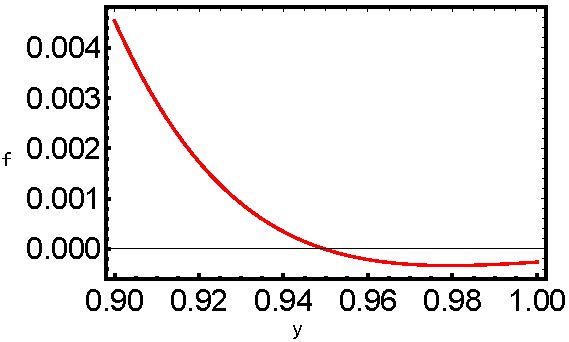
\includegraphics[scale=1]{f-b-2d.pdf}
			\caption{splitting function $f$ from diagram b in Fig.~\ref{fig:diagrams}} 
			\label{f-b-Dterm}
		\end{center}
	\end{figure}
	that means integral below will contain divergence 
	\[
	\int_{-\xi}^{\xi}d(1-y)f(y,\xi,t)\frac{1}{1-y}D(\frac{x}{\xi},t)
	\]
	We can define such a function 
	\[
	F(y,x,\xi,t)=f(y,\xi,t)\frac{1}{1-y}D(\frac{x}{\xi},t)
	\] 
	which gives a figure with certain $x\ \xi\ t$ like Fig.~\ref{F-b-Dterm}
	\begin{figure}[htbp]
		\begin{center}
			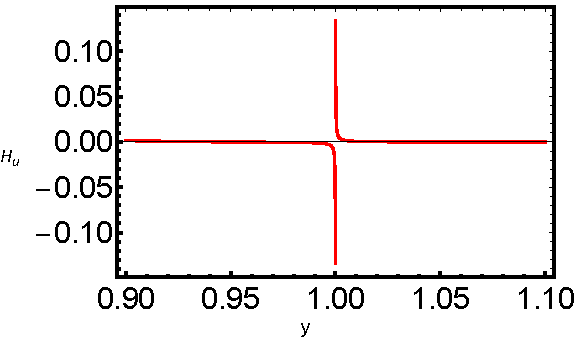
\includegraphics[scale=1]{hd-b-2d.pdf}
			\caption{figure of $F(y,x,\xi,t)$ at $(x,\xi,t)=(-0.01,0.1,-1)$} 
			\label{F-b-Dterm}
		\end{center}
	\end{figure}
	In Fig.~\ref{F-b-Dterm}, the $F(y,x,\xi,t)$ looks like a odd function which divergence can be canceled.We can use a simpler form of $F(y,x,\xi,t)$ to show the idea.For integral like
	\[
	\int_{b_{2}}^{b_{1}}dx\frac{A(x)}{x}
	\]
	
	we can expand the numerator $A(x)$ around $x=0$ 
	\begin{align*}
		\int_{b_{2}}^{b_{1}}dx\frac{A(x)}{x} & =\int_{b_{2}}^{b_{1}}dx\frac{1}{x}(a_{0}+a_{1}x+a_{2}x^{2}+...)\\
		& =\int_{b_{2}}^{b_{1}}dx\frac{1}{x}a_{0}+\int_{b_{2}}^{b_{1}}dxa_{1}+\int_{b_{2}}^{b_{1}}dxa_{2}x+...\\
		& +\int_{b_{2}}^{b_{1}}dxa_{n}x^{n-1}+...
	\end{align*} 
	Now only the first term contains a divergence when the value of $b_{1}b_{2}$ is small and  $b_{1}<0<b_{2}$. And since the $\frac{1}{x}$ is odd we can cancel the divergence like 
	\[
	\int_{-\xi}^{\xi}dx\frac{1}{x}=0
	\]
	Of course this is not a serious proof of the convergence of this integral, but this shows that this integral may not be divergent and we can check this with some numerical calculation.
	For the actual integral in convolution calculation, which is 
	\[
	\int_{-\xi}^{\xi}d(1-y)f(y,\xi,t)\frac{1}{1-y}D(\frac{x}{\xi},t)
	\]
	we do this change to it
	\begin{gather*}
		\int_{-\xi}^{\xi}d(1-y)f(y,\xi,t)\frac{1}{1-y}D(\frac{x}{\xi},t)\\
		=\int_{1-\xi}^{1+\xi}d(y)f(y,\xi,t)\frac{1}{1-y}D(\frac{x}{\xi},t)\\
		=\int_{1-\xi}^{1-a}d(y)f(y,\xi,t)\frac{1}{1-y}D(\frac{x}{\xi},t)+\int_{1-a}^{1+a}d(y)f(y,\xi,t)\frac{1}{1-y}D(\frac{x}{\xi},t)+\int_{1+a}^{1+\xi}d(y)f(y,\xi,t)\frac{1}{1-y}D(\frac{x}{\xi},t)
	\end{gather*}
	where $0<a<\xi$. So the first and third integral do not contain divergence because they do not cross $y=1$. If the divergence can be canceled, we would have \[
	\int_{1-a}^{1+a}d(y)f(y,\xi,t)\frac{1}{1-y}D(\frac{x}{\xi},t)=0
	\]
	This can be checked by numerical calculation. Firstly, if $a$ is small enough, we have \[
	\underset{a\rightarrow0}{\textrm{Lim}}\int_{1-a}^{1+a}d(y)f(y,\xi,t)\frac{1}{1-y}D(\frac{x}{\xi},t)=0\] because of
	\begin{align*}
		\int_{1-a}^{1+a}dy\frac{f(y,\xi,t)}{1-y}D(\frac{x}{\xi},t) & =\int_{1-a}^{1}dy\frac{f(y,\xi,t)}{1-y}D(\frac{x}{\xi},t)+\int_{1}^{1+a}dy\frac{f(y,\xi,t)}{1-y}D(\frac{x}{\xi},t)\\
		\underset{a\rightarrow0}{\textrm{Lim}}\int_{1-a}^{1}dyf(y,\xi,t)D(\frac{x}{\xi},t) & =a*\frac{f(1-a,\xi,t)}{1-(1-a)}D(\frac{x}{\xi},t)\\
		& =-|f(1,\xi,t)D(\frac{x}{\xi},t)|\\
		\underset{a\rightarrow0}{\textrm{Lim}}\int_{1}^{1+a}dyf(y,\xi,t)D(\frac{x}{\xi},t) & =a*\frac{f(1+a,\xi,t)}{(1+a)-1}D(\frac{x}{\xi},t)\\
		& =|f(1,\xi,t)D(\frac{x}{\xi},t)|
	\end{align*}
	Of course this is the limit but if we set $a_{n}$ as a small enough value to make  \[
	\int_{1-a_{n}}^{1+a_{n}}d(y)f(y,\xi,t)\frac{1}{1-y}D(\frac{x}{\xi},t)=0
	\] and chose $a_{0}>a_{1}>a_{2}>...>a_{n-1}>a_{n}$ as some certain value smaller than $\xi$. For $a_{0}>a_{1}$, we have 
	\begin{multline*}
		\int_{1-a_{0}}^{1+a_{0}}dy\frac{f(y,\xi,t)}{1-y}D(\frac{x}{\xi},t)=\\
		\int_{1-a_{0}}^{1-a_{1}}dy\frac{f(y,\xi,t)}{1-y}D(\frac{x}{\xi},t)+\int_{1-a_{1}}^{1+a_{1}}dy\frac{f(y,\xi,t)}{1-y}D(\frac{x}{\xi},t)+\int_{1+a_{1}}^{1+a_{0}}dy\frac{f(y,\xi,t)}{1-y}D(\frac{x}{\xi},t)
	\end{multline*}
	Repeat this, the integral will become
	\begin{multline*}
		\int_{1-a_{0}}^{1+a_{0}}dy\frac{f(y,\xi,t)}{1-y}D(\frac{x}{\xi},t)=\\
		\int_{1-a_{0}}^{1-a_{1}}dy\frac{f(y,\xi,t)}{1-y}D(\frac{x}{\xi},t)+\int_{1-a_{1}}^{1+a_{1}}dy\frac{f(y,\xi,t)}{1-y}D(\frac{x}{\xi},t)+\int_{1+a_{1}}^{1+a_{0}}dy\frac{f(y,\xi,t)}{1-y}D(\frac{x}{\xi},t)\\
		=\int_{1-a_{0}}^{1-a_{1}}dy\frac{f(y,\xi,t)}{1-y}D(\frac{x}{\xi},t)+\int_{1-a_{1}}^{1-a_{2}}dy\frac{f(y,\xi,t)}{1-y}D(\frac{x}{\xi},t)+\int_{1-a_{2}}^{1-a_{3}}dy\frac{f(y,\xi,t)}{1-y}D(\frac{x}{\xi},t)\\
		+\int_{1-a_{n-1}}^{1-a_{n}}dy\frac{f(y,\xi,t)}{1-y}D(\frac{x}{\xi},t)+\int_{1-a_{n}}^{1+a_{n}}dy\frac{f(y,\xi,t)}{1-y}D(\frac{x}{\xi},t)+\int_{1+a_{n}}^{1+a_{n-1}}dy\frac{f(y,\xi,t)}{1-y}D(\frac{x}{\xi},t)\\
		+\int_{1+a_{3}}^{1+a_{2}}dy\frac{f(y,\xi,t)}{1-y}D(\frac{x}{\xi},t)+\int_{1+a_{2}}^{1+a_{1}}dy\frac{f(y,\xi,t)}{1-y}D(\frac{x}{\xi},t)+\int_{1+a_{1}}^{1+a_{0}}dy\frac{f(y,\xi,t)}{1-y}D(\frac{x}{\xi},t)
	\end{multline*}
	And if we can check each integral like 
	\[\int_{1-a_{0}}^{1-a_{1}}dy\frac{f(y,\xi,t)}{1-y}D(\frac{x}{\xi},t)+\int_{1+a_{1}}^{1+a_{0}}dy\frac{f(y,\xi,t)}{1-y}D(\frac{x}{\xi},t)=0\] the equation above is $0$. And this is equal to the $I(a)$ below  
	\[
	I(a)=\int_{1-\xi}^{1-a}d(y)f(y,\xi,t)\frac{1}{1-y}D(\frac{x}{\xi},t)+\int_{1+a}^{1+\xi}d(y)f(y,\xi,t)\frac{1}{1-y}D(\frac{x}{\xi},t)
	\]
	has same result with different $a$ which is 
	\begin{gather*}
		\int_{1-\xi}^{1-a_{1}}dy\frac{f(y,\xi,t)}{1-y}D(\frac{x}{\xi},t)+\int_{1+a_{1}}^{1+\xi}dy\frac{f(y,\xi,t)}{1-y}D(\frac{x}{\xi},t)\\
		=\int_{1-\xi}^{1-a_{0}}dy\frac{f(y,\xi,t)}{1-y}D(\frac{x}{\xi},t)+\int_{1-a_{0}}^{1-a_{1}}dy\frac{f(y,\xi,t)}{1-y}D(\frac{x}{\xi},t)\\
		+\int_{1+a_{0}}^{1+\xi}dy\frac{f(y,\xi,t)}{1-y}D(\frac{x}{\xi},t)+\int_{1+a_{1}}^{1+a_{0}}dy\frac{f(y,\xi,t)}{1-y}D(\frac{x}{\xi},t)\\
		=\int_{1-\xi}^{1-a_{0}}dy\frac{f(y,\xi,t)}{1-y}D(\frac{x}{\xi},t)+\int_{1+a_{0}}^{1+\xi}dy\frac{f(y,\xi,t)}{1-y}D(\frac{x}{\xi},t)\\
		+\int_{1-a_{0}}^{1-a_{1}}dy\frac{f(y,\xi,t)}{1-y}D(\frac{x}{\xi},t)+\int_{1+a_{1}}^{1+a_{0}}dy\frac{f(y,\xi,t)}{1-y}D(\frac{x}{\xi},t)
	\end{gather*}
	The result for diagram b is 
	\begin{align*}
		I(0.01) & =0.00002284065045\\
		I(10^{-4}) & =0.00001941004441\\
		I(10^{-6}) & =0.0000193752819\\
		I(10^{-8}) & =0.0000193749343\\
		I(10^{-10}) & =0.0000193749308
	\end{align*}
	So this may imply that the divergence in D-term can be canceled. Then we can add D-term in convolution calculation. 
	Only with D-term we can get GPD result similar to meson loop case. Otherwise the GPD in baryon loop will give smooth curve around $x=\xi$. The figures below are the original result from convolution calculation. In Fig.~\ref{H-b-nD} and Fig.~\ref{E-b-nD} there are the figures of GPD result from diagram b without D-term in the input GPD and GDA. These two curves are smooth.
	And in Fig.~\ref{H-b-D} and Fig~\ref{E-b-D}, we have corresponding figure of GPD with D-term in input which have a change between DGLAP and ERBL region which is more similar to the previous meson loop calculation.
	\begin{figure}[h]
		\begin{center}
			\includegraphics[scale=0.5]{H3d-b-noD.pdf}
			\caption{$H(x,\xi,t)$ from diagram b without D-term at $(\xi,t)=(0.1,-1)$} 
			\label{H-b-nD-3d}
		\end{center}
	\end{figure}
	
	\begin{figure}[h]
		\begin{center}
			\includegraphics[scale=0.5]{E3d-b-noD.pdf}
			\caption{$E(x,\xi,t)$ from diagram b without D-term at $(\xi,t)=(0.1,-1)$} 
			\label{E-b-nD-3d}
		\end{center}
	\end{figure}
	
	\begin{figure}[h]
		\begin{center}
			\includegraphics[scale=0.5]{H3d-b-D.pdf}
			\caption{$H(x,\xi,t)$ from diagram b with D-term at $(\xi,t)=(0.1,-1)$} 
			\label{H-b-D-3d}
		\end{center}
	\end{figure}
	
	\begin{figure}[h]
		\begin{center}
			\includegraphics[scale=0.5]{E3d-b-D.pdf}
			\caption{$E(x,\xi,t)$ from diagram b with D-term at $(\xi,t)=(0.1,-1)$} 
			\label{E-b-D-3d}
		\end{center}
	\end{figure}
	
	\begin{figure}[htbp]
		\begin{center}
			\includegraphics[scale=0.5]{H2d-b-noD.pdf}
			\caption{$H(x,\xi,t)$ from diagram b without D-term at $(\xi,t)=(0.1,-1)$} 
			\label{H-b-nD}
		\end{center}
	\end{figure}
	
	\begin{figure}[h]
		\begin{center}
			\includegraphics[scale=0.5]{E2d-b-noD.pdf}
			\caption{$E(x,\xi,t)$ from diagram b without D-term at $(\xi,t)=(0.1,-1)$} 
			\label{E-b-nD}
		\end{center}
	\end{figure}
	
	\begin{figure}[h]
		\begin{center}
			\includegraphics[scale=0.5]{H2d-b-D.pdf}
			\caption{$H(x,\xi,t)$ from diagram b with D-term at $(\xi,t)=(0.1,-1)$} 
			\label{H-b-D}
		\end{center}
	\end{figure}
	
	\begin{figure}[h]
		\begin{center}
			\includegraphics[scale=0.5]{E2d-b-D.pdf}
			\caption{$E(x,\xi,t)$ from diagram b with D-term at $(\xi,t)=(0.1,-1)$} 
			\label{E-b-D}
		\end{center}
	\end{figure}
	For KR diagrams when the external field couples to the baryon the input is polarized GPD which do not have extra D-term in double distribution represent. But when the external field couples to the meson, GPD of pion has D-term and the convolution formula for D-term is 
	\[
	\int_{-\xi}^{\xi}d(y)f(y,\xi,t)\frac{1}{y}D(\frac{x}{\xi},t)
	\]
	which asks the splitting function satisfy $f(0)=0$. And for KR diagrams we can not have this feature of splitting function. So we also need to use same method as the rainbow diagrams. The result with D-term for diagram f is
	In Fig.~\ref{H-f-nD} at $x=0.1=\xi$, the curve is not smooth. The reason is the number of  points I chose in calculating the GDA part is too small and we can not give the correct curve. 
	\begin{figure}[h]
		\begin{center}
			\includegraphics[scale=0.5]{H3d-f-noD.pdf}
			\caption{$H(x,\xi,t)$ from diagram f without D-term at $(\xi,t)=(0.1,-1)$} 
			\label{H-f-nD-3d}
		\end{center}
	\end{figure}
	\begin{figure}[h]
		\begin{center}
			\includegraphics[scale=0.5]{E3d-f-noD.pdf}
			\caption{$E(x,\xi,t)$ from diagram f without D-term at $(\xi,t)=(0.1,-1)$} 
			\label{E-f-nD-3d}
		\end{center}
	\end{figure}
	\begin{figure}[h]
		\begin{center}
			\includegraphics[scale=0.5]{H3d-f-D.pdf}
			\caption{$H(x,\xi,t)$ from diagram f with D-term at $(\xi,t)=(0.1,-1)$} 
			\label{H-f-D-3d}
		\end{center}
	\end{figure}
	\begin{figure}[h]
		\begin{center}
			\includegraphics[scale=0.5]{E3d-f-D.pdf}
			\caption{$E(x,\xi,t)$ from diagram f with D-term at $(\xi,t)=(0.1,-1)$} 
			\label{E-f-D-3d}
		\end{center}
	\end{figure}
	\begin{figure}[h]
		\begin{center}
			\includegraphics[scale=0.5]{H2d-f-noD.pdf}
			\caption{$H(x,\xi,t)$ from diagram f without D-term at $(\xi,t)=(0.1,-1)$} 
			\label{H-f-nD}
		\end{center}
	\end{figure}
	\begin{figure}[h]
		\begin{center}
			\includegraphics[scale=0.5]{E2d-f-noD.pdf}
			\caption{$E(x,\xi,t)$ from diagram f without D-term at $(\xi,t)=(0.1,-1)$} 
			\label{E-f-nD}
		\end{center}
	\end{figure}
	\begin{figure}[h]
		\begin{center}
			\includegraphics[scale=0.5]{H2d-f-D.pdf}
			\caption{$H(x,\xi,t)$ from diagram f with D-term at $(\xi,t)=(0.1,-1)$} 
			\label{H-f-D}
		\end{center}
	\end{figure}
	\begin{figure}[h]
		\begin{center}
			\includegraphics[scale=0.5]{E2d-f-D.pdf}
			\caption{$E(x,\xi,t)$ from diagram f with D-term at $(\xi,t)=(0.1,-1)$} 
			\label{E-f-D}
		\end{center}
	\end{figure}
	\begin{figure}[h]
		\begin{center}
			\includegraphics[scale=0.5]{H2d-f-polar.pdf}
			\caption{$H(x,\xi,t)$ from diagram f with baryon input at $(\xi,t)=(0.1,-1)$} 
			\label{H-f-polar}
		\end{center}
	\end{figure}
	\begin{figure}[h]
		\begin{center}
			\includegraphics[scale=0.5]{E2d-f-polar.pdf}
			\caption{$E(x,\xi,t)$ from diagram f  with baryon input at $(\xi,t)=(0.1,-1)$} 
			\label{E-f-polar}
		\end{center}
	\end{figure}
	\section{result of GPD}
	Now we can get the final result of GPD from the diagrams in Fig.~\ref{fig:diagrams}. 
	\subsection{rainbow diagram}
	For diagrams b,c,n,o,p,q in Fig.~\ref{fig:diagrams}, the rainbow diagrams where the external field couple to the baryon, since the input function is baryon GPD, there is no anti quark which means we do not have $x<-\xi$ region of GPD. Using the symmetry of hadronic configurations from previous paper, the input GPD of other baryon is related to the GPD of proton then we have the GPD result from different channel. For example, in diagram b, the GPD result of d quark is 
	\begin{figure}[h]
		\begin{center}
			\includegraphics[scale=0.5]{H-b-2d-717.pdf}
			\caption{$H(x,\xi,t)$ from diagram b at $(\xi,t)=(0.1,-1)$} 
			\label{H-f-nD}
		\end{center}
	\end{figure}
	\begin{figure}[h]
		\begin{center}
			\includegraphics[scale=0.5]{E-b-2d-717.pdf}
			\caption{$E(x,\xi,t)$ from diagram b at $(\xi,t)=(0.1,-1)$} 
			\label{H-f-nD}
		\end{center}
	\end{figure}
	
	\subsection{KR diagram}
	For diagram d,e,f,g,r,s,t,u in Fig.~\ref{fig:diagrams}, the KR diagram, I calculate the GPD using the new definition where the external field couple to the meson and this makes the GPD result of KR diagrams like with the meson loop case have anti quark contribution. For diagram f, the u quark GPD is  
	\begin{figure}[h]
		\begin{center}
			\includegraphics[scale=0.5]{H-f-2d-717.pdf}
			\caption{$H(x,\xi,t)$ from diagram f at $(\xi,t)=(0.1,-1)$} 
			\label{H-f-nD}
		\end{center}
	\end{figure}
	\begin{figure}[h]
		\begin{center}
			\includegraphics[scale=0.5]{E-f-2d-717.pdf}
			\caption{$E(x,\xi,t)$ from diagram f at $(\xi,t)=(0.1,-1)$} 
			\label{H-f-nD}
		\end{center}
	\end{figure}
	
	\section{form factor result}
	With the nonzero skewness GPD,  we can get electromagnetic and gravitation form factor of different quark in proton. 
	\subsection{electromagnetic form factor}
	\subsubsection{baryon case}
	For those baryon loop diagrams in Fig.~\ref{fig:rainbowdiagrams}, the GPD $H$ of u,d quark, the $H_{u}\ H_{d}$ are given as Fig.~\ref{Hu-bar} ~\ref{Eu-bar}  ~\ref{Hd-bar} ~\ref{Ed-bar}  
	\begin{figure}[h]
		\begin{center}
			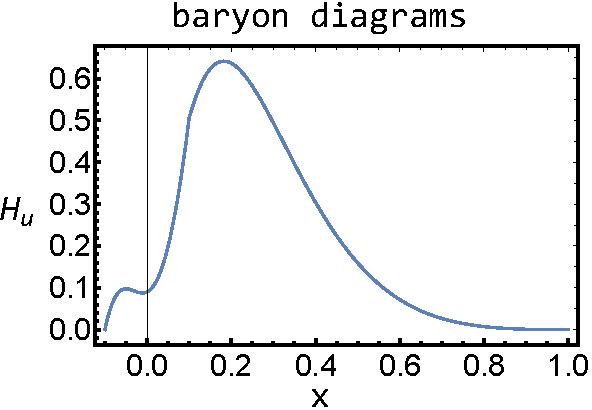
\includegraphics[scale=0.5]{Hu-baryon-2d.pdf}
			\caption{$H^{u}(x,\xi,t)$ from baryon loop diagram at $(\xi,t)=(0.1,-1)$} 
			\label{Hu-bar}
		\end{center}
	\end{figure}
	\begin{figure}[h]
		\begin{center}
			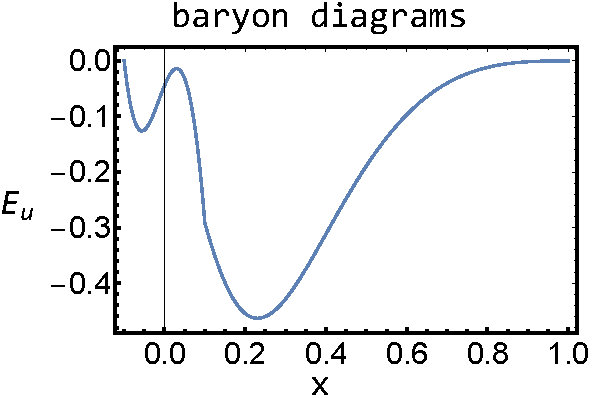
\includegraphics[scale=0.5]{Eu-baryon-2d.pdf}
			\caption{$E^{u}(x,\xi,t)$ from baryon loop diagram at $(\xi,t)=(0.1,-1)$} 
			\label{Eu-bar}
		\end{center}
	\end{figure}  
	\begin{figure}[h]
		\begin{center}
			\includegraphics[scale=0.5]{Hd-baryon-2d.pdf}
			\caption{$H^{d}(x,\xi,t)$ from baryon loop diagram at $(\xi,t)=(0.1,-1)$} 
			\label{Hd-bar}
		\end{center}
	\end{figure}
	\begin{figure}[h]
		\begin{center}
			\includegraphics[scale=0.5]{Ed-baryon-2d.pdf}
			\caption{$E^{d}(x,\xi,t)$ from baryon loop diagram at $(\xi,t)=(0.1,-1)$} 
			\label{Ed-bar}
		\end{center}
	\end{figure}  
	And the corresponding form factor is 
	\begin{align}
		& F^{u}_{1}=0.217765 \ F^{u}_{2}=-0.0199994 \\
		& F^{d}_{1}=0.129507 \ F^{d}_{2}=0.0594396
	\end{align}
	\subsubsection{KR diagram}
	For KR diagrams the contribution to GPD of ud quark is Fig.~\ref{Hu-kr} ~\ref{Eu-kr}  ~\ref{Hd-kr} ~\ref{Ed-kr}  
	\begin{figure}[h]
		\begin{center}
			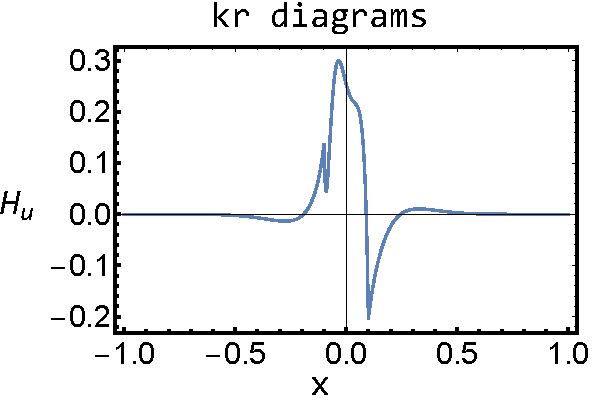
\includegraphics[scale=0.5]{Hu-kr-2d.pdf}
			\caption{$H^{u}(x,\xi,t)$ from kr diagram at $(\xi,t)=(0.1,-1)$} 
			\label{Hu-kr}
		\end{center}
	\end{figure}
	\begin{figure}[h]
		\begin{center}
			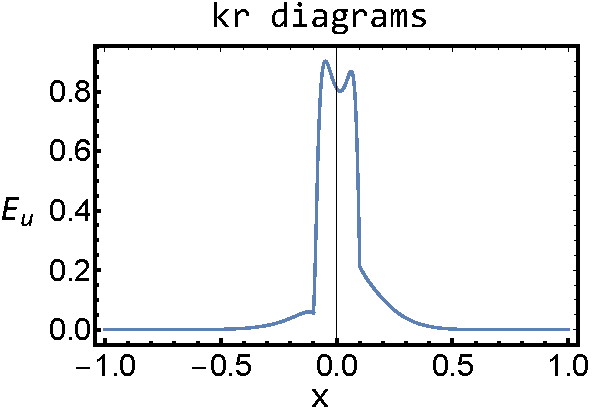
\includegraphics[scale=0.5]{Eu-kr-2d.pdf}
			\caption{$E^{u}(x,\xi,t)$ from kr diagram at $(\xi,t)=(0.1,-1)$} 
			\label{Eu-kr}
		\end{center}
	\end{figure}  
	\begin{figure}[h]
		\begin{center}
			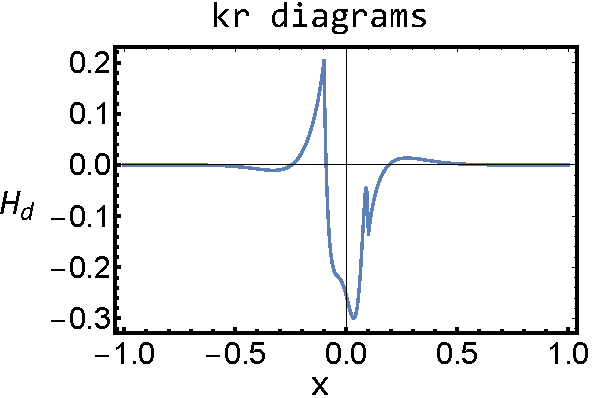
\includegraphics[scale=0.5]{Hd-kr-2d.pdf}
			\caption{$H^{d}(x,\xi,t)$ from kr diagram at $(\xi,t)=(0.1,-1)$} 
			\label{Hd-kr}
		\end{center}
	\end{figure}
	\begin{figure}[h]
		\begin{center}
			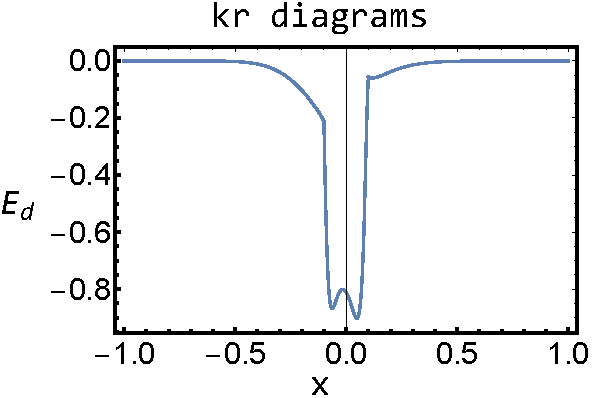
\includegraphics[scale=0.5]{Ed-kr-2d.pdf}
			\caption{$E^{d}(x,\xi,t)$ from kr diagram at $(\xi,t)=(0.1,-1)$} 
			\label{Ed-kr}
		\end{center}
	\end{figure}  
	The corresponding form factor which contains both the quark and anti quark contribution is 
	\begin{align}
		& F^{u}_{1}=0.03176  \ F^{u}_{2}=0.184198 \\
		& F^{d}_{1}= -0.03176\ F^{d}_{2}=-0.184198
	\end{align}
	\subsection{tadpole}
	For tadpole diagrams the contribution to GPD of ud quark is Fig.~\ref{Hu-tad} ~\ref{Eu-tad}  ~\ref{Hd-tad} ~\ref{Ed-tad}  
	\begin{figure}[h]
		\begin{center}
			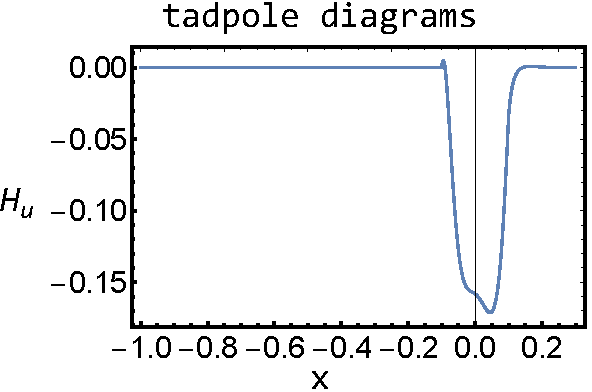
\includegraphics[scale=0.5]{Hu-tadpole-2d.pdf}
			\caption{$H^{u}(x,\xi,t)$ from tadpole diagram at $(\xi,t)=(0.1,-1)$} 
			\label{Hu-tad}
		\end{center}
	\end{figure}
	\begin{figure}[h]
		\begin{center}
			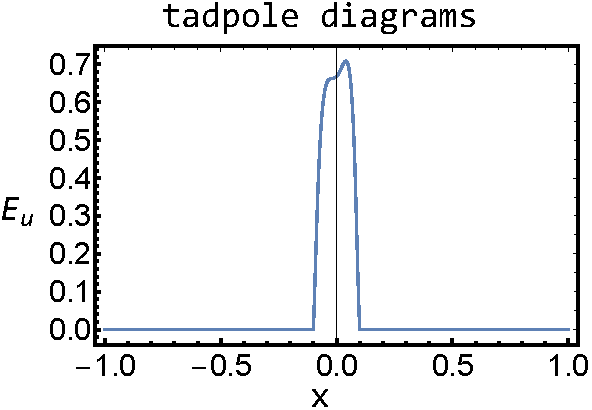
\includegraphics[scale=0.5]{Eu-tadpole-2d.pdf}
			\caption{$E^{u}(x,\xi,t)$ from tadpole diagram at $(\xi,t)=(0.1,-1)$} 
			\label{Eu-tad}
		\end{center}
	\end{figure}  
	\begin{figure}[h]
		\begin{center}
			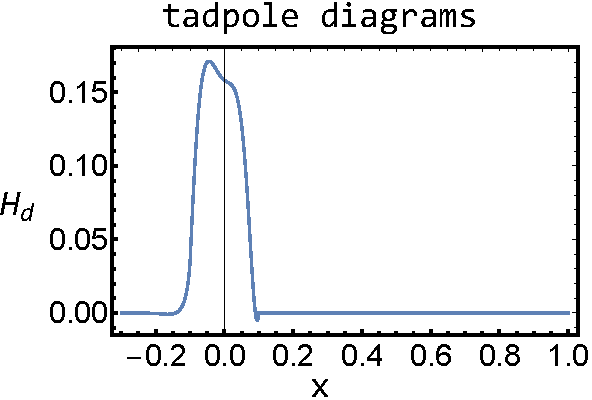
\includegraphics[scale=0.5]{Hd-tadpole-2d.pdf}
			\caption{$H^{d}(x,\xi,t)$ from tadpole diagram at $(\xi,t)=(0.1,-1)$} 
			\label{Hd-tad}
		\end{center}
	\end{figure}
	\begin{figure}[h]
		\begin{center}
			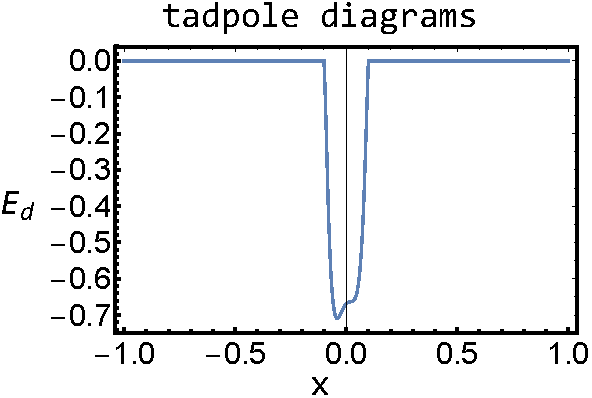
\includegraphics[scale=0.5]{Ed-tadpole-2d.pdf}
			\caption{$E^{d}(x,\xi,t)$ from tadpole diagram at $(\xi,t)=(0.1,-1)$} 
			\label{Ed-tad}
		\end{center}
	\end{figure}  
	The corresponding form factor which contains both the quark and anti quark contribution is 
	\begin{align}
		& F^{u}_{1}=-0.0250034  \ F^{u}_{2}=0.109394 \\
		& F^{d}_{1}=0.0250034\ F^{d}_{2}=-0.109394
	\end{align}
	\subsection{$\bar{d}-\bar{u}$ result}
	Like what Fangcheng done in the meson loop case I calculate the contribution of $F_{1}^{\bar{d}-\bar{u}}$ and $F_{2}^{\bar{d}-\bar{u}}$ from the KR and tadpole diagram. 
	The result of $\bar{d}-\bar{u}$ now is showed in Fig ~\ref{F1udbar} ~\ref{F2udbar}.
	I try to check if the $d$ quark contribution from polarized GPD can cancel with the $\bar{d}$ quark from pion. Only consider the sea quark contribution in polarize GPD case, which is corresponding to the pion loop contribution, the result is showed in Fig ~\ref{F1udbarpo} ~\ref{F2udbarpo}.
	\begin{figure}[h]
		\begin{center}
			\includegraphics[scale=0.5]{F1-823.pdf}
			\caption{result of $F^{\bar{d}-\bar{u}}_{1}$ the red line is contribution of meson loop and in black line I add KR and tadpole diagram} 
			\label{F1udbar}
		\end{center}
	\end{figure}
	\begin{figure}[h]
		\begin{center}
			\includegraphics[scale=0.5]{F2-823.pdf}
			\caption{result of $F^{\bar{d}-\bar{u}}_{2
				}$ the red line is contribution of meson loop and in black line I add KR and tadpole diagram} 
			\label{F2udbar}
		\end{center}
	\end{figure} 
	
	\begin{figure}[h]
		\begin{center}
			\includegraphics[scale=0.5]{F1udbar-polar.pdf}
			\caption{result of $F^{\bar{d}-\bar{u}}_{1}$ the red curve is contribution of meson loop and in black curve I add KR and tadpole diagram and in the blue curve I add the contribution from polarized GPD in KR and tadpole diagram} 
			\label{F1udbarpo}
		\end{center}
	\end{figure}
	\begin{figure}[h]
		\begin{center}
			\includegraphics[scale=0.5]{F2udbar-polar.pdf}
			\caption{result of $F^{\bar{d}-\bar{u}}_{2
				}$ the red line is contribution of meson loop and in black line I add KR and tadpole diagram} 
			\label{F2udbarpo}
		\end{center}
	\end{figure} 
	In Fig~\ref{dubar},~\ref{xdubar},~\ref{dcu}, I give the result of x dependence of $\bar{d}-\bar{u}$ from different method. The main problem is that no matter we add the KR and tadpole diagrams or not, the two curves are close to each other, which means the difference is in $\delta$ term contribution.
	\begin{figure}[h]
		\begin{center}
			\includegraphics[scale=0.5]{xdubar.pdf}
			\caption{$x(\bar{d}(x)-\bar{u}(x))$,the blue curve is $x(\bar{d}(x)-\bar{u}(x))$ from meson loop, the red curve is $x(\bar{d}(x)-\bar{u}(x))$ from KR and tadpole diagram and the black curve is the whole result } 
			\label{xdubar}
		\end{center}
	\end{figure}
	\begin{figure}[h]
		\begin{center}
			\includegraphics[scale=0.5]{dubar.pdf}
			\caption{$\bar{d}(x)-\bar{u}(x)$,the blue curve is $\bar{d}(x)-\bar{u}(x)$ from meson loop, the red curve is $\bar{d}(x)-\bar{u}(x)$ from KR and tadpole diagram and the black curve is the whole result } 
			\label{dubar}
		\end{center}
	\end{figure}
	\begin{figure}[h]
		\begin{center}
			\includegraphics[scale=0.5]{dcu.pdf}
			\caption{$\frac{\bar{d}(x)}{\bar{u}(x)}$,the blue curve is $\frac{\bar{d}(x)}{\bar{u}(x)}$ from meson loop, the black curve is the whole result of meson and KR diagrams} 
			\label{dcu}
		\end{center}
	\end{figure}
	
	\begin{figure}[h]
		\begin{center}
			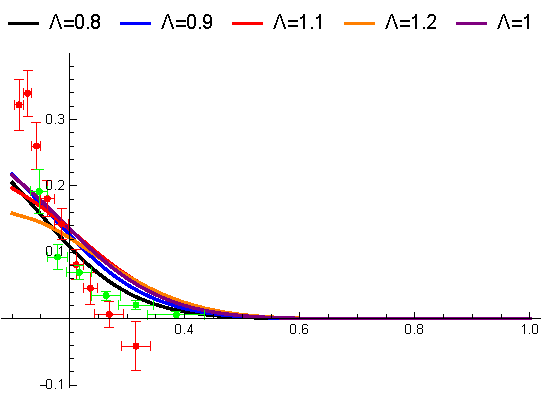
\includegraphics[scale=0.8]{dubar5L.pdf}
			\caption{$\bar{d}(x)-\bar{u}(x)$ result with different $\Lambda$} 
			\label{5Lambda}
		\end{center}
	\end{figure}
	
	\begin{figure}[h]
		\begin{center}
			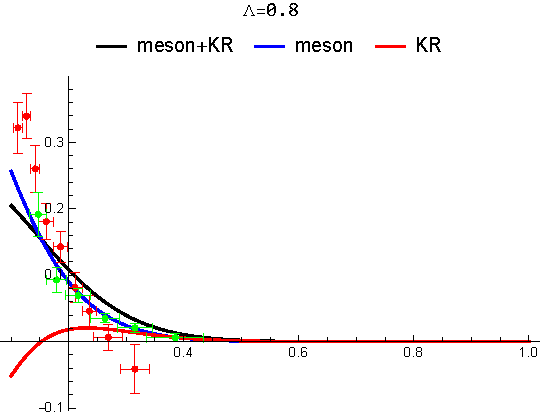
\includegraphics[scale=0.8]{dubarL08.pdf}
			\caption{$\bar{d}(x)-\bar{u}(x)$ result with $\Lambda=0.8Gev$ and different curves represent different diagram.} 
			\label{08Lambda}
		\end{center}
	\end{figure}
	
	\begin{figure}[h]
		\begin{center}
			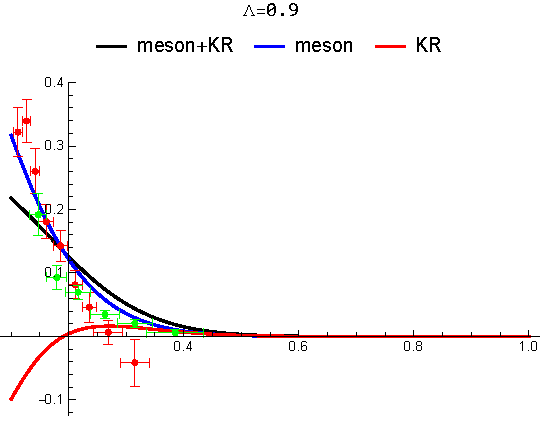
\includegraphics[scale=0.8]{dubarL09.pdf}
			\caption{$\bar{d}(x)-\bar{u}(x)$ result with $\Lambda=0.9Gev$ and different curves represent different diagram.} 
			\label{09Lambda}
		\end{center}
	\end{figure}
	
	\begin{figure}[h]
		\begin{center}
			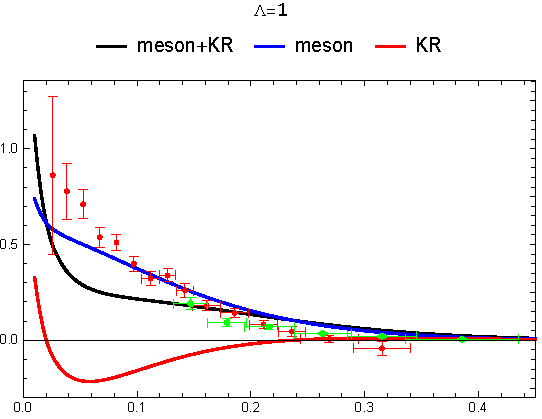
\includegraphics[scale=0.8]{dubarL1.pdf}
			\caption{$\bar{d}(x)-\bar{u}(x)$ result with $\Lambda=1.0Gev$ and different curves represent different diagram.} 
			\label{1Lambda}
		\end{center}
	\end{figure}
	
	\begin{figure}[h]
		\begin{center}
			\includegraphics[scale=0.8]{dubarL11.pdf}
			\caption{$\bar{d}(x)-\bar{u}(x)$ result with $\Lambda=1.1Gev$ and different curves represent different diagram.} 
			\label{11Lambda}
		\end{center}
	\end{figure}
	\begin{figure}[h]
		\begin{center}
			\includegraphics[scale=0.8]{dubarL12.pdf}
			\caption{$\bar{d}(x)-\bar{u}(x)$ result with $\Lambda=1.2Gev$ and different curves represent different diagram.} 
			\label{12Lambda}
		\end{center}
	\end{figure}
	
	\begin{figure}[h]
		\begin{center}
			\includegraphics[scale=0.8]{xdubarL5.pdf}
			\caption{$x\bar{d}(x)-x\bar{u}(x)$ result with different $\Lambda$} 
			\label{x5Lambda}
		\end{center}
	\end{figure}
	
	\begin{figure}[h]
		\begin{center}
			\includegraphics[scale=0.8]{xdubarL08.pdf}
			\caption{$x\bar{d}(x)-x\bar{u}(x)$ result with $\Lambda=0.8Gev$ and different curves represent different diagram.} 
			\label{x08Lambda}
		\end{center}
	\end{figure}
	
	\begin{figure}[h]
		\begin{center}
			\includegraphics[scale=0.8]{xdubarL09.pdf}
			\caption{$x\bar{d}(x)-x\bar{u}(x)$ result with $\Lambda=0.9Gev$ and different curves represent different diagram.} 
			\label{x09Lambda}
		\end{center}
	\end{figure}
	
	\begin{figure}[h]
		\begin{center}
			\includegraphics[scale=0.8]{xdubarL1.pdf}
			\caption{$x\bar{d}(x)-x\bar{u}(x)$ result with $\Lambda=1.0Gev$ and different curves represent different diagram.} 
			\label{x1Lambda}
		\end{center}
	\end{figure}
	
	\begin{figure}[h]
		\begin{center}
			\includegraphics[scale=0.8]{xdubarL11.pdf}
			\caption{$x\bar{d}(x)-x\bar{u}(x)$ result with $\Lambda=1.1Gev$ and different curves represent different diagram.} 
			\label{x11Lambda}
		\end{center}
	\end{figure}
	\begin{figure}[h]
		\begin{center}
			\includegraphics[scale=0.8]{xdubarL12.pdf}
			\caption{$x\bar{d}(x)-x\bar{u}(x)$ result with $\Lambda=1.2Gev$ and different curves represent different diagram.} 
			\label{x12Lambda}
		\end{center}
	\end{figure}
	\subsection{gravitation form factor}
	The first order moment of GPD is corresponding to the gravitation form factor of quark. In, our calculation, the first order moment, which is $\int_{-1}^{1}xH^{u}(x,\xi,t)dx$ since the convolution formula, is divided into two part 
	\[\int_{-\xi}^{\xi}xH^{u}(x,\xi,t)dx+\int_{\xi}^{1}xH^{u}(x,\xi,t)dx\]
	In DGLAP region we have 
	\begin{align*}
		\int_{\xi}^{1}xH^{u}(x,\xi,t)dx & =\int_{\xi}^{1}xdx\int_{x}^{1}d\bar{y}\frac{1}{\bar{y}}f(\bar{y},\xi,t)H_{in}^{u}(\frac{x}{\bar{y}},\frac{\xi}{\bar{y}},t)\\
		& =\int_{\xi}^{1}d\bar{y}f(\bar{y},\xi,t)\int_{\xi}^{\bar{y}}dx\frac{x}{\bar{y}}H_{in}^{u}(\frac{x}{\bar{y}},\frac{\xi}{\bar{y}},t)\\
		& =\int_{\xi}^{1}d\bar{y}\bar{y}f(\bar{y},\xi,t)\int_{\frac{\xi}{\bar{y}}}^{1}d\frac{x}{\bar{y}}\frac{x}{\bar{y}}H_{in}^{u}(\frac{x}{\bar{y}},\frac{\xi}{\bar{y}},t)
	\end{align*}
	In ERBL region which contains two part with different input, firstly the GPD part is 
	\begin{align*}
		\int_{-\xi}^{\xi}xH^{u}(x,\xi,t)dx & =\int_{-\xi}^{\xi}xdx\int_{\xi}^{1}d\bar{y}\frac{1}{\bar{y}}f(\bar{y},\xi,t)H_{in}^{u}(\frac{x}{\bar{y}},\frac{\xi}{\bar{y}},t)\\
		& =\int_{\xi}^{1}d\bar{y}f(\bar{y},\xi,t)\int_{-\xi}^{\xi}dx\frac{x}{\bar{y}}H_{in}^{u}(\frac{x}{\bar{y}},\frac{\xi}{\bar{y}},t)\\
		& =\int_{\xi}^{1}d\bar{y}\bar{y}f(\bar{y},\xi,t)\int_{\frac{-\xi}{\bar{y}}}^{\frac{\xi}{\bar{y}}}d\frac{x}{\bar{y}}\frac{x}{\bar{y}}H_{in}^{u}(\frac{x}{\bar{y}},\frac{\xi}{\bar{y}},t)
	\end{align*}
	In GDA part we have 
	\begin{align*}
		\int_{-\xi}^{\xi}xH^{u}(x,\xi,t)dx & =\int_{-\xi}^{\xi}xdx\int_{-\xi}^{\xi}d\bar{y}\frac{1}{\bar{y}}f(\bar{y},\xi,t)\frac{1}{2}\Phi(\eta,z,t)\\
		& =\int_{-\xi}^{\xi}d\bar{y}\frac{1}{\bar{y}}f(\bar{y},\xi,t)\int_{-\xi}^{\xi}x\frac{1}{2}\Phi(\eta,z,t)dx\\
		& =\int_{-\xi}^{\xi}d\bar{y}\frac{1}{\bar{y}}f(\bar{y},\xi,t)\xi^{2}\int_{0}^{1}d\eta(2\eta-1)\Phi(\eta,z,t)
	\end{align*}
	\begin{align*}
		\int_{0}^{1}dz(2z-1)^{n-1}\Phi(z,\eta,t) & =\underset{i=0,even}{\overset{n-1}{\Sigma}}2^{i}(2\eta-1)^{2-i}A_{i}^{n}+2^{n}C^{n}\\
		& =\underset{i=0,even}{\overset{n-1}{\Sigma}}2^{i}(\frac{\bar{y}}{\xi})^{2-i}A_{i}^{n}+2^{n}C^{n}
	\end{align*}
	Notice in the second line of the equation above, the definition of $z,\eta$ in $\Phi(z,\eta,t)$ should be same with the convolution formula where $2z-1=\frac{x}{\xi},\ 2\eta-1=\frac{\bar{y}}{\xi}$ 
	\begin{align*}
		\int_{-1}^{1}dxx^{n-1}H^{u}_{in}(x,\xi,t)=\underset{i=0,even}{\overset{n-1}{\Sigma}}(2\xi)^{i}A^{n}_{i}(t)+(2\xi)^{n}C^{n}(t)|_{n\ even}
	\end{align*}
	\begin{align*}
		\int_{-\xi}^{\xi}xH^{u}(x,\xi,t)dx & =\int_{-\xi}^{\xi}d\bar{y}\frac{1}{\bar{y}}f(\bar{y},\xi,t)\xi^{2}*((\frac{\bar{y}}{\xi})^{2}A_{0}^{2}+2^{2}C^{2})\\
		& =\int_{-\xi}^{\xi}d\bar{y}\bar{y}f(\bar{y},\xi,t)(\frac{\xi}{\bar{y}})^{2}*((\frac{\bar{y}}{\xi})^{2}A_{0}^{2}+2^{2}C^{2})\\
		& =\int_{-\xi}^{\xi}d\bar{y}\bar{y}f(\bar{y},\xi,t)(A_{0}^{2}+(\frac{2\xi}{\bar{y}})^{2}C^{2})\\
		& =\int_{-\xi}^{\xi}d\bar{y}\bar{y}f(\bar{y},\xi,t)\int_{-\frac{\xi}{\bar{y}}}^{1}dzzH_{in}^{u}(z,\frac{\xi}{\bar{y}},t)
	\end{align*}
	So the complete result is 
	
	\begin{align*}
		\int_{-\xi}^{1}xH^{u}(x,\xi,t)dx & =\int_{\xi}^{1}xH^{u}(x,\xi,t)dx+\int_{-\xi}^{\xi}xH_{gpd}^{u}(x,\xi,t)dx+\int_{-\xi}^{\xi}xH_{gda}^{u}(x,\xi,t)dx\\
		& =\int_{\xi}^{1}d\bar{y}\bar{y}f(\bar{y},\xi,t)\int_{\frac{\xi}{\bar{y}}}^{1}dzzH_{in}^{u}(z,\frac{\xi}{\bar{y}},t)+\int_{\xi}^{1}d\bar{y}\bar{y}f(\bar{y},\xi,t)\int_{-\frac{\xi}{\bar{y}}}^{\frac{\xi}{\bar{y}}}dzzH_{in}^{u}(z,\frac{\xi}{\bar{y}},t)\\
		& +\int_{-\xi}^{\xi}d\bar{y}\bar{y}f(\bar{y},\xi,t)\int_{-\frac{\xi}{\bar{y}}}^{1}dzzH_{in}^{u}(z,\frac{\xi}{\bar{y}},t)\\
		& =\int_{-\xi}^{1}d\bar{y}\bar{y}f(\bar{y},\xi,t)\int_{-\frac{\xi}{\bar{y}}}^{1}dzzH_{in}^{u}(z,\frac{\xi}{\bar{y}},t)
	\end{align*}
	
	The input GPD part can be calculated directly notice the result of input GPD contains $\bar{y}$ now but the $\delta$ term in splitting function has a problem
	\[
	\int_{\xi}^{1}d\bar{y}\bar{y}f(\bar{y},\xi,t)\rightarrow\int_{\xi}^{1}d\bar{y}\bar{y}f_{\delta}(\bar{y},\xi,t)\delta(y)
	\]
	\begin{align*}
		\int_{\xi}^{1}d\bar{y}(1-y)f_{\delta}(y,\xi,t)\delta(y) & =\int_{\xi}^{1}d\bar{y}f_{\delta}(y,\xi,t)\delta(y)-\int_{\xi}^{1}d\bar{y}yf_{\delta}(y,\xi,t)\delta(y)\\
		\int_{\xi}^{1}d\bar{y}yf_{\delta}(y,\xi,t)\delta(y) & =\int_{0}^{1-\xi}dyyf_{\delta}(y,\xi,t)\delta(y)
	\end{align*}
	When we get the $\delta$ term, like introduced above, we change the projection $A$ and $B$ to be
	\begin{align}
		& \frac{1}{D_{\phi}(k) D^{4}_{\Lambda}(k)}\\
		& \frac{k^{-}}{D_{\phi}(k) D^{4}_{\Lambda}(k)}
	\end{align}
	For the second term, we need to cancel the $k^{-}$ in the numerator  
	\begin{align}
		\frac{k^{-}}{D_{\phi}(k)D_{\Lambda}^{4}(k)} & =\frac{1}{k^{+}}\frac{k^{+}k^{-}}{D_{\phi}(k)D_{\Lambda}^{4}(k)}\\
		& =\frac{1}{k^{+}}\frac{D_{\phi}(k)+(k^{\perp})^{2}+m_{\phi}^{2}}{D_{\phi}(k)D_{\Lambda}^{4}(k)}\\
		& \rightarrow\frac{1}{k^{+}}*\delta(k^{+})\delta(\frac{k^{+}}{P^{+}}-y)\\
		& \rightarrow\frac{1}{y}*\delta(y)
	\end{align}
	This term does not contribute to the GPD and the lowest order moment but when we calculate the first order moment the $y$ in the denominator cancel and give contribution to gravitation form factor.
	\[
	\int_{0}^{1-\xi}dyyf_{\delta}(y,\xi,t)\delta(y)\rightarrow\int dy*y*\frac{1}{y}\delta(y)
	\]
	
\end{document}
